% Options for packages loaded elsewhere
\PassOptionsToPackage{unicode}{hyperref}
\PassOptionsToPackage{hyphens}{url}
%
\documentclass[
]{article}
\usepackage{lmodern}
\usepackage{amssymb,amsmath}
\usepackage{ifxetex,ifluatex}
\ifnum 0\ifxetex 1\fi\ifluatex 1\fi=0 % if pdftex
  \usepackage[T1]{fontenc}
  \usepackage[utf8]{inputenc}
  \usepackage{textcomp} % provide euro and other symbols
\else % if luatex or xetex
  \usepackage{unicode-math}
  \defaultfontfeatures{Scale=MatchLowercase}
  \defaultfontfeatures[\rmfamily]{Ligatures=TeX,Scale=1}
\fi
% Use upquote if available, for straight quotes in verbatim environments
\IfFileExists{upquote.sty}{\usepackage{upquote}}{}
\IfFileExists{microtype.sty}{% use microtype if available
  \usepackage[]{microtype}
  \UseMicrotypeSet[protrusion]{basicmath} % disable protrusion for tt fonts
}{}
\makeatletter
\@ifundefined{KOMAClassName}{% if non-KOMA class
  \IfFileExists{parskip.sty}{%
    \usepackage{parskip}
  }{% else
    \setlength{\parindent}{0pt}
    \setlength{\parskip}{6pt plus 2pt minus 1pt}}
}{% if KOMA class
  \KOMAoptions{parskip=half}}
\makeatother
\usepackage{xcolor}
\IfFileExists{xurl.sty}{\usepackage{xurl}}{} % add URL line breaks if available
\IfFileExists{bookmark.sty}{\usepackage{bookmark}}{\usepackage{hyperref}}
\hypersetup{
  pdftitle={PSA: Markov Sick-Sicker model in R},
  pdfauthor={The DARTH workgroup},
  hidelinks,
  pdfcreator={LaTeX via pandoc}}
\urlstyle{same} % disable monospaced font for URLs
\usepackage[margin=1in]{geometry}
\usepackage{color}
\usepackage{fancyvrb}
\newcommand{\VerbBar}{|}
\newcommand{\VERB}{\Verb[commandchars=\\\{\}]}
\DefineVerbatimEnvironment{Highlighting}{Verbatim}{commandchars=\\\{\}}
% Add ',fontsize=\small' for more characters per line
\usepackage{framed}
\definecolor{shadecolor}{RGB}{248,248,248}
\newenvironment{Shaded}{\begin{snugshade}}{\end{snugshade}}
\newcommand{\AlertTok}[1]{\textcolor[rgb]{0.94,0.16,0.16}{#1}}
\newcommand{\AnnotationTok}[1]{\textcolor[rgb]{0.56,0.35,0.01}{\textbf{\textit{#1}}}}
\newcommand{\AttributeTok}[1]{\textcolor[rgb]{0.77,0.63,0.00}{#1}}
\newcommand{\BaseNTok}[1]{\textcolor[rgb]{0.00,0.00,0.81}{#1}}
\newcommand{\BuiltInTok}[1]{#1}
\newcommand{\CharTok}[1]{\textcolor[rgb]{0.31,0.60,0.02}{#1}}
\newcommand{\CommentTok}[1]{\textcolor[rgb]{0.56,0.35,0.01}{\textit{#1}}}
\newcommand{\CommentVarTok}[1]{\textcolor[rgb]{0.56,0.35,0.01}{\textbf{\textit{#1}}}}
\newcommand{\ConstantTok}[1]{\textcolor[rgb]{0.00,0.00,0.00}{#1}}
\newcommand{\ControlFlowTok}[1]{\textcolor[rgb]{0.13,0.29,0.53}{\textbf{#1}}}
\newcommand{\DataTypeTok}[1]{\textcolor[rgb]{0.13,0.29,0.53}{#1}}
\newcommand{\DecValTok}[1]{\textcolor[rgb]{0.00,0.00,0.81}{#1}}
\newcommand{\DocumentationTok}[1]{\textcolor[rgb]{0.56,0.35,0.01}{\textbf{\textit{#1}}}}
\newcommand{\ErrorTok}[1]{\textcolor[rgb]{0.64,0.00,0.00}{\textbf{#1}}}
\newcommand{\ExtensionTok}[1]{#1}
\newcommand{\FloatTok}[1]{\textcolor[rgb]{0.00,0.00,0.81}{#1}}
\newcommand{\FunctionTok}[1]{\textcolor[rgb]{0.00,0.00,0.00}{#1}}
\newcommand{\ImportTok}[1]{#1}
\newcommand{\InformationTok}[1]{\textcolor[rgb]{0.56,0.35,0.01}{\textbf{\textit{#1}}}}
\newcommand{\KeywordTok}[1]{\textcolor[rgb]{0.13,0.29,0.53}{\textbf{#1}}}
\newcommand{\NormalTok}[1]{#1}
\newcommand{\OperatorTok}[1]{\textcolor[rgb]{0.81,0.36,0.00}{\textbf{#1}}}
\newcommand{\OtherTok}[1]{\textcolor[rgb]{0.56,0.35,0.01}{#1}}
\newcommand{\PreprocessorTok}[1]{\textcolor[rgb]{0.56,0.35,0.01}{\textit{#1}}}
\newcommand{\RegionMarkerTok}[1]{#1}
\newcommand{\SpecialCharTok}[1]{\textcolor[rgb]{0.00,0.00,0.00}{#1}}
\newcommand{\SpecialStringTok}[1]{\textcolor[rgb]{0.31,0.60,0.02}{#1}}
\newcommand{\StringTok}[1]{\textcolor[rgb]{0.31,0.60,0.02}{#1}}
\newcommand{\VariableTok}[1]{\textcolor[rgb]{0.00,0.00,0.00}{#1}}
\newcommand{\VerbatimStringTok}[1]{\textcolor[rgb]{0.31,0.60,0.02}{#1}}
\newcommand{\WarningTok}[1]{\textcolor[rgb]{0.56,0.35,0.01}{\textbf{\textit{#1}}}}
\usepackage{graphicx,grffile}
\makeatletter
\def\maxwidth{\ifdim\Gin@nat@width>\linewidth\linewidth\else\Gin@nat@width\fi}
\def\maxheight{\ifdim\Gin@nat@height>\textheight\textheight\else\Gin@nat@height\fi}
\makeatother
% Scale images if necessary, so that they will not overflow the page
% margins by default, and it is still possible to overwrite the defaults
% using explicit options in \includegraphics[width, height, ...]{}
\setkeys{Gin}{width=\maxwidth,height=\maxheight,keepaspectratio}
% Set default figure placement to htbp
\makeatletter
\def\fps@figure{htbp}
\makeatother
\setlength{\emergencystretch}{3em} % prevent overfull lines
\providecommand{\tightlist}{%
  \setlength{\itemsep}{0pt}\setlength{\parskip}{0pt}}
\setcounter{secnumdepth}{-\maxdimen} % remove section numbering

\title{PSA: Markov Sick-Sicker model in R}
\author{The DARTH workgroup}
\date{}

\begin{document}
\maketitle

Developed by the Decision Analysis in R for Technologies in Health
(DARTH) workgroup:

Fernando Alarid-Escudero, PhD (1)

Eva A. Enns, MS, PhD (2)

M.G. Myriam Hunink, MD, PhD (3,4)

Hawre J. Jalal, MD, PhD (5)

Eline M. Krijkamp, MSc (3)

Petros Pechlivanoglou, PhD (6,7)

Alan Yang, MSc (7)

In collaboration of:

\begin{enumerate}
\def\labelenumi{\arabic{enumi}.}
\tightlist
\item
  Division of Public Administration, Center for Research and Teaching in
  Economics (CIDE), Aguascalientes, Mexico
\item
  University of Minnesota School of Public Health, Minneapolis, MN, USA
\item
  Erasmus MC, Rotterdam, The Netherlands
\item
  Harvard T.H. Chan School of Public Health, Boston, USA
\item
  University of Pittsburgh Graduate School of Public Health, Pittsburgh,
  PA, USA
\item
  University of Toronto, Toronto ON, Canada
\item
  The Hospital for Sick Children, Toronto ON, Canada
\end{enumerate}

Please cite our publications when using this code:

\begin{itemize}
\item
  Jalal H, Pechlivanoglou P, Krijkamp E, Alarid-Escudero F, Enns E,
  Hunink MG. An Overview of R in Health Decision Sciences. Med Decis
  Making. 2017; 37(3): 735-746.
  \url{https://journals.sagepub.com/doi/abs/10.1177/0272989X16686559}
\item
  Krijkamp EM, Alarid-Escudero F, Enns EA, Jalal HJ, Hunink MGM,
  Pechlivanoglou P. Microsimulation modeling for health decision
  sciences using R: A tutorial. Med Decis Making. 2018;38(3):400--22.
  \url{https://journals.sagepub.com/doi/abs/10.1177/0272989X18754513}
\item
  Krijkamp EM, Alarid-Escudero F, Enns E, Pechlivanoglou P, Hunink MM,
  Jalal H. A Multidimensional Array Representation of State-Transition
  Model Dynamics. Med Decis Making. 2020 Online first.
  \url{https://doi.org/10.1177/0272989X19893973}
\item
  Alarid-Escudero, F., Krijkamp, E. M., Enns, E. A., Hunink, M. G. M.,
  Pechlivanoglou, P., \& Jalal, H. (2020). Cohort state-transition
  models in R: From conceptualization to implementation.
  arXiv:2001.07824v1, 1--31. \url{http://arxiv.org/abs/2001.07824}
\item
  Alarid-Escudero, F., Enns, E. A., Kuntz, K. M., Michaud, T. L., \&
  Jalal, H. (2019). ``Time Traveling Is Just Too Dangerous'' But Some
  Methods Are Worth Revisiting: The Advantages of Expected Loss Curves
  Over Cost-Effectiveness Acceptability Curves and Frontier. Value in
  Health, 22(5), 611--618.
  \url{https://doi.org/10.1016/j.jval.2019.02.008}
\end{itemize}

Copyright 2017, THE HOSPITAL FOR SICK CHILDREN AND THE COLLABORATING
INSTITUTIONS. All rights reserved in Canada, the United States and
worldwide. Copyright, trademarks, trade names and any and all associated
intellectual property are exclusively owned by THE HOSPITAL FOR Sick
CHILDREN and the collaborating institutions. These materials may be
used, reproduced, modified, distributed and adapted with proper
attribution.

\newpage

\begin{Shaded}
\begin{Highlighting}[]
\KeywordTok{rm}\NormalTok{(}\DataTypeTok{list =} \KeywordTok{ls}\NormalTok{())      }\CommentTok{# clear memory (removes all the variables from the workspace)}
\end{Highlighting}
\end{Shaded}

\hypertarget{load-packages}{%
\section{01 Load packages}\label{load-packages}}

\begin{Shaded}
\begin{Highlighting}[]
\ControlFlowTok{if}\NormalTok{ (}\OperatorTok{!}\KeywordTok{require}\NormalTok{(}\StringTok{'pacman'}\NormalTok{)) \{}
  \KeywordTok{install.packages}\NormalTok{(}\StringTok{'pacman'}\NormalTok{)}
\NormalTok{\}}
\KeywordTok{library}\NormalTok{(pacman) }\CommentTok{# use this package to conveniently install other packages}
\CommentTok{# load (install if required) packages from CRAN}
\KeywordTok{p_load}\NormalTok{(}\StringTok{"here"}\NormalTok{, }\StringTok{"dplyr"}\NormalTok{, }\StringTok{"devtools"}\NormalTok{, }\StringTok{"scales"}\NormalTok{, }\StringTok{"ellipse"}\NormalTok{, }\StringTok{"ggplot2"}\NormalTok{, }\StringTok{"lazyeval"}\NormalTok{, }
       \StringTok{"igraph"}\NormalTok{, }\StringTok{"truncnorm"}\NormalTok{, }\StringTok{"ggraph"}\NormalTok{, }\StringTok{"reshape2"}\NormalTok{, }\StringTok{"knitr"}\NormalTok{, }\StringTok{"stringr"}\NormalTok{, }\StringTok{"reshape2"}\NormalTok{)                                            }
\CommentTok{# load (install if required) packages from GitHub}
\CommentTok{# install_github("DARTH-git/dampack", force = TRUE) Uncomment if there is a newer version}
\CommentTok{# install_github("DARTH-git/dectree", force = TRUE) Uncomment if there is a newer version}
\CommentTok{# install_github("annaheath/EVSI", force = TRUE) #Uncomment if there is a newer version}
\KeywordTok{p_load_gh}\NormalTok{(}\StringTok{"DARTH-git/dampack"}\NormalTok{, }\StringTok{"DARTH-git/dectree"}\NormalTok{)}
\KeywordTok{p_load_gh}\NormalTok{(}\StringTok{"annaheath/EVSI"}\NormalTok{)}
\end{Highlighting}
\end{Shaded}

\hypertarget{load-functions}{%
\section{02 Load functions}\label{load-functions}}

\begin{Shaded}
\begin{Highlighting}[]
\KeywordTok{source}\NormalTok{(}\StringTok{"Functions.R"}\NormalTok{)}
\end{Highlighting}
\end{Shaded}

\hypertarget{input-model-parameters}{%
\section{03 Input model parameters}\label{input-model-parameters}}

\begin{Shaded}
\begin{Highlighting}[]
\CommentTok{# Strategy names}
\NormalTok{v_names_str <-}\StringTok{ }\KeywordTok{c}\NormalTok{(}\StringTok{"No Treatment"}\NormalTok{, }\StringTok{"Treatment"}\NormalTok{) }

\CommentTok{# Number of strategies}
\NormalTok{n_str <-}\StringTok{ }\KeywordTok{length}\NormalTok{(v_names_str)}

\CommentTok{# Markov model parameters}
\NormalTok{age     <-}\StringTok{ }\DecValTok{25}                       \CommentTok{# age at baseline}
\NormalTok{max_age <-}\StringTok{ }\DecValTok{55}                       \CommentTok{# maximum age of follow up}
\NormalTok{n_t     <-}\StringTok{ }\NormalTok{max_age }\OperatorTok{-}\StringTok{ }\NormalTok{age            }\CommentTok{# time horizon, number of cycles}
\NormalTok{v_n     <-}\StringTok{ }\KeywordTok{c}\NormalTok{(}\StringTok{"H"}\NormalTok{, }\StringTok{"S1"}\NormalTok{, }\StringTok{"S2"}\NormalTok{, }\StringTok{"D"}\NormalTok{)  }\CommentTok{# the 4 states of the model: Healthy (H), }
                                    \CommentTok{# Sick (S1), Sicker (S2), Dead (D)}
\NormalTok{n_s     <-}\StringTok{ }\KeywordTok{length}\NormalTok{(v_n)              }\CommentTok{# number of health states }

\CommentTok{# Transition probabilities (per cycle)}
\NormalTok{p_HD    <-}\StringTok{ }\FloatTok{0.005}           \CommentTok{# probability to die when healthy}
\NormalTok{p_HS1   <-}\StringTok{ }\FloatTok{0.15}              \CommentTok{# probability to become sick when healthy}
\NormalTok{p_S1H   <-}\StringTok{ }\FloatTok{0.5}               \CommentTok{# probability to become healthy when sick}
\NormalTok{p_S1S2  <-}\StringTok{ }\FloatTok{0.105}             \CommentTok{# probability to become sicker when sick}
\NormalTok{hr_S1   <-}\StringTok{ }\DecValTok{3}                 \CommentTok{# hazard ratio of death in sick vs healthy}
\NormalTok{hr_S2   <-}\StringTok{ }\DecValTok{10}                \CommentTok{# hazard ratio of death in sicker vs healthy }
\NormalTok{r_HD    <-}\StringTok{ }\OperatorTok{-}\StringTok{ }\KeywordTok{log}\NormalTok{(}\DecValTok{1} \OperatorTok{-}\StringTok{ }\NormalTok{p_HD) }\CommentTok{# rate of death in healthy}
\NormalTok{r_S1D   <-}\StringTok{ }\NormalTok{hr_S1 }\OperatorTok{*}\StringTok{ }\NormalTok{r_HD      }\CommentTok{# rate of death in sick}
\NormalTok{r_S2D   <-}\StringTok{ }\NormalTok{hr_S2 }\OperatorTok{*}\StringTok{ }\NormalTok{r_HD      }\CommentTok{# rate of death in sicker}
\NormalTok{p_S1D   <-}\StringTok{ }\DecValTok{1} \OperatorTok{-}\StringTok{ }\KeywordTok{exp}\NormalTok{(}\OperatorTok{-}\NormalTok{r_S1D) }\CommentTok{# probability to die in sick}
\NormalTok{p_S2D   <-}\StringTok{ }\DecValTok{1} \OperatorTok{-}\StringTok{ }\KeywordTok{exp}\NormalTok{(}\OperatorTok{-}\NormalTok{r_S2D) }\CommentTok{# probability to die in sicker}

\CommentTok{# Cost and utility inputs }
\NormalTok{c_H     <-}\StringTok{ }\DecValTok{2000}   \CommentTok{# cost of remaining one cycle in the healthy state}
\NormalTok{c_S1    <-}\StringTok{ }\DecValTok{4000}   \CommentTok{# cost of remaining one cycle in the sick state}
\NormalTok{c_S2    <-}\StringTok{ }\DecValTok{15000}  \CommentTok{# cost of remaining one cycle in the sicker state}
\NormalTok{c_trt   <-}\StringTok{ }\DecValTok{12000}  \CommentTok{# cost of treatment(per cycle)}
\NormalTok{c_D     <-}\StringTok{ }\DecValTok{0}      \CommentTok{# cost of being in the death state}
\NormalTok{u_H     <-}\StringTok{ }\DecValTok{1}      \CommentTok{# utility when healthy}
\NormalTok{u_S1    <-}\StringTok{ }\FloatTok{0.75}   \CommentTok{# utility when sick}
\NormalTok{u_S2    <-}\StringTok{ }\FloatTok{0.5}    \CommentTok{# utility when sicker}
\NormalTok{u_D     <-}\StringTok{ }\DecValTok{0}      \CommentTok{# utility when dead}
\NormalTok{u_trt   <-}\StringTok{ }\FloatTok{0.95}   \CommentTok{# utility when being treated}

\CommentTok{# Discounting factor}
\NormalTok{d_r     <-}\StringTok{ }\FloatTok{0.03} \CommentTok{# equal discount of costs and QALYs by 3%}
\CommentTok{# calculate discount weights for costs for each cycle based on discount rate d_c}
\NormalTok{v_dwc   <-}\StringTok{ }\DecValTok{1} \OperatorTok{/}\StringTok{ }\NormalTok{(}\DecValTok{1} \OperatorTok{+}\StringTok{ }\NormalTok{d_r) }\OperatorTok{^}\StringTok{ }\NormalTok{(}\DecValTok{0}\OperatorTok{:}\NormalTok{n_t) }
\CommentTok{# calculate discount weights for effectiveness for each cycle based on discount rate d_e}
\NormalTok{v_dwe   <-}\StringTok{ }\DecValTok{1} \OperatorTok{/}\StringTok{ }\NormalTok{(}\DecValTok{1} \OperatorTok{+}\StringTok{ }\NormalTok{d_r) }\OperatorTok{^}\StringTok{ }\NormalTok{(}\DecValTok{0}\OperatorTok{:}\NormalTok{n_t) }
\end{Highlighting}
\end{Shaded}

\hypertarget{define-and-initialize-matrices-and-vectors}{%
\section{04 Define and initialize matrices and
vectors}\label{define-and-initialize-matrices-and-vectors}}

\hypertarget{cohort-trace}{%
\subsection{04.1 Cohort trace}\label{cohort-trace}}

\begin{Shaded}
\begin{Highlighting}[]
\CommentTok{# create the markov trace matrix M capturing the proportion of the cohort }
\CommentTok{# in each state at each cycle}
\NormalTok{m_M_notrt <-}\StringTok{ }\NormalTok{m_M_trt <-}\StringTok{ }\KeywordTok{matrix}\NormalTok{(}\OtherTok{NA}\NormalTok{, }
                                \DataTypeTok{nrow     =}\NormalTok{ n_t }\OperatorTok{+}\StringTok{ }\DecValTok{1}\NormalTok{, }\DataTypeTok{ncol =}\NormalTok{ n_s,}
                                \DataTypeTok{dimnames =} \KeywordTok{list}\NormalTok{(}\KeywordTok{paste}\NormalTok{(}\StringTok{"cycle"}\NormalTok{, }\DecValTok{0}\OperatorTok{:}\NormalTok{n_t, }\DataTypeTok{sep =} \StringTok{" "}\NormalTok{), v_n))}

\KeywordTok{head}\NormalTok{(m_M_notrt) }\CommentTok{# show first 6 rows of the matrix }
\end{Highlighting}
\end{Shaded}

\begin{verbatim}
##          H S1 S2  D
## cycle 0 NA NA NA NA
## cycle 1 NA NA NA NA
## cycle 2 NA NA NA NA
## cycle 3 NA NA NA NA
## cycle 4 NA NA NA NA
## cycle 5 NA NA NA NA
\end{verbatim}

\begin{Shaded}
\begin{Highlighting}[]
\CommentTok{# The cohort starts as healthy}
\NormalTok{m_M_notrt[}\DecValTok{1}\NormalTok{, ] <-}\StringTok{ }\NormalTok{m_M_trt[}\DecValTok{1}\NormalTok{, ] <-}\StringTok{ }\KeywordTok{c}\NormalTok{(}\DecValTok{1}\NormalTok{, }\DecValTok{0}\NormalTok{, }\DecValTok{0}\NormalTok{, }\DecValTok{0}\NormalTok{) }\CommentTok{# initiate first cycle of cohort trace }
\end{Highlighting}
\end{Shaded}

\hypertarget{transition-probability-matrix}{%
\subsection{04.2 Transition probability
matrix}\label{transition-probability-matrix}}

\begin{Shaded}
\begin{Highlighting}[]
\CommentTok{# create the transition probability matrix for NO treatment (notrt)}
\NormalTok{m_P_notrt  <-}\StringTok{ }\KeywordTok{matrix}\NormalTok{(}\DecValTok{0}\NormalTok{,}
                     \DataTypeTok{nrow =}\NormalTok{ n_s,}
                     \DataTypeTok{ncol =}\NormalTok{ n_s,}
                     \DataTypeTok{dimnames =} \KeywordTok{list}\NormalTok{(v_n, v_n)) }\CommentTok{# name the columns and rows of the matrix}
\NormalTok{m_P_notrt}
\end{Highlighting}
\end{Shaded}

\begin{verbatim}
##    H S1 S2 D
## H  0  0  0 0
## S1 0  0  0 0
## S2 0  0  0 0
## D  0  0  0 0
\end{verbatim}

Fill in the transition probability matrix:

\begin{Shaded}
\begin{Highlighting}[]
\CommentTok{# from Healthy}
\NormalTok{m_P_notrt[}\StringTok{"H"}\NormalTok{, }\StringTok{"H"}\NormalTok{]   <-}\StringTok{ }\DecValTok{1} \OperatorTok{-}\StringTok{ }\NormalTok{(p_HS1 }\OperatorTok{+}\StringTok{ }\NormalTok{p_HD)}
\NormalTok{m_P_notrt[}\StringTok{"H"}\NormalTok{, }\StringTok{"S1"}\NormalTok{]  <-}\StringTok{ }\NormalTok{p_HS1}
\NormalTok{m_P_notrt[}\StringTok{"H"}\NormalTok{, }\StringTok{"D"}\NormalTok{]   <-}\StringTok{ }\NormalTok{p_HD}
\CommentTok{# from Sick}
\NormalTok{m_P_notrt[}\StringTok{"S1"}\NormalTok{, }\StringTok{"H"}\NormalTok{]  <-}\StringTok{ }\NormalTok{p_S1H}
\NormalTok{m_P_notrt[}\StringTok{"S1"}\NormalTok{, }\StringTok{"S1"}\NormalTok{] <-}\StringTok{ }\DecValTok{1} \OperatorTok{-}\StringTok{ }\NormalTok{(p_S1H }\OperatorTok{+}\StringTok{ }\NormalTok{p_S1S2 }\OperatorTok{+}\StringTok{ }\NormalTok{p_S1D)}
\NormalTok{m_P_notrt[}\StringTok{"S1"}\NormalTok{, }\StringTok{"S2"}\NormalTok{] <-}\StringTok{ }\NormalTok{p_S1S2}
\NormalTok{m_P_notrt[}\StringTok{"S1"}\NormalTok{, }\StringTok{"D"}\NormalTok{]  <-}\StringTok{ }\NormalTok{p_S1D}
\CommentTok{# from Sicker}
\NormalTok{m_P_notrt[}\StringTok{"S2"}\NormalTok{, }\StringTok{"S2"}\NormalTok{] <-}\StringTok{ }\DecValTok{1} \OperatorTok{-}\StringTok{ }\NormalTok{p_S2D}
\NormalTok{m_P_notrt[}\StringTok{"S2"}\NormalTok{, }\StringTok{"D"}\NormalTok{]  <-}\StringTok{ }\NormalTok{p_S2D}
\CommentTok{# from Dead}
\NormalTok{m_P_notrt[}\StringTok{"D"}\NormalTok{, }\StringTok{"D"}\NormalTok{]   <-}\StringTok{ }\DecValTok{1}

\CommentTok{# check rows add up to 1}
\KeywordTok{rowSums}\NormalTok{(m_P_notrt)}
\end{Highlighting}
\end{Shaded}

\begin{verbatim}
##  H S1 S2  D 
##  1  1  1  1
\end{verbatim}

\begin{Shaded}
\begin{Highlighting}[]
\CommentTok{# create transition probability matrix for treatment same as no treatment}
\NormalTok{m_P_trt <-}\StringTok{ }\NormalTok{m_P_notrt}
\end{Highlighting}
\end{Shaded}

\hypertarget{run-markov-model}{%
\section{05 Run Markov model}\label{run-markov-model}}

\begin{Shaded}
\begin{Highlighting}[]
\ControlFlowTok{for}\NormalTok{ (t }\ControlFlowTok{in} \DecValTok{1}\OperatorTok{:}\NormalTok{n_t)\{     }\CommentTok{# loop through the number of cycles}
\NormalTok{  m_M_notrt[t }\OperatorTok{+}\StringTok{ }\DecValTok{1}\NormalTok{, ] <-}\StringTok{ }\KeywordTok{t}\NormalTok{(m_M_notrt[t, ]) }\OperatorTok\StringTok{ }\NormalTok{m_P_notrt }\CommentTok{# estimate the Markov trace }
                                                        \CommentTok{# for the next cycle (t + 1)}
\NormalTok{  m_M_trt[t }\OperatorTok{+}\StringTok{ }\DecValTok{1}\NormalTok{, ]   <-}\StringTok{ }\KeywordTok{t}\NormalTok{(m_M_trt[t, ])    }\OperatorTok\StringTok{ }\NormalTok{m_P_trt    }\CommentTok{# estimate the Markov trace }
                                                           \CommentTok{# for the next cycle (t + 1)}
\NormalTok{\} }\CommentTok{# close the loop}

\KeywordTok{head}\NormalTok{(m_M_notrt)  }\CommentTok{# show the first 6 lines of the matrix}
\end{Highlighting}
\end{Shaded}

\begin{verbatim}
##                 H        S1         S2          D
## cycle 0 1.0000000 0.0000000 0.00000000 0.00000000
## cycle 1 0.8450000 0.1500000 0.00000000 0.00500000
## cycle 2 0.7890250 0.1837612 0.01575000 0.01146377
## cycle 3 0.7586067 0.1881968 0.03427491 0.01892157
## cycle 4 0.7351211 0.1853199 0.05235988 0.02719916
## cycle 5 0.7138373 0.1807036 0.06925860 0.03620055
\end{verbatim}

\hypertarget{compute-and-plot-epidemiological-outcomes}{%
\section{06 Compute and Plot Epidemiological
Outcomes}\label{compute-and-plot-epidemiological-outcomes}}

\hypertarget{cohort-trace-1}{%
\subsection{06.1 Cohort trace}\label{cohort-trace-1}}

\begin{Shaded}
\begin{Highlighting}[]
\CommentTok{# create a plot of the data}
\KeywordTok{matplot}\NormalTok{(m_M_notrt, }\DataTypeTok{type =} \StringTok{'l'}\NormalTok{, }
        \DataTypeTok{ylab =} \StringTok{"Probability of state occupancy"}\NormalTok{,}
        \DataTypeTok{xlab =} \StringTok{"Cycle"}\NormalTok{,}
        \DataTypeTok{main =} \StringTok{"Cohort Trace"}\NormalTok{)             }
\CommentTok{# add a legend to the graph}
\KeywordTok{legend}\NormalTok{(}\StringTok{"topright"}\NormalTok{, v_n, }\DataTypeTok{col =} \DecValTok{1}\OperatorTok{:}\NormalTok{n_s, }\DataTypeTok{lty =} \DecValTok{1}\OperatorTok{:}\NormalTok{n_s, }\DataTypeTok{bty =} \StringTok{"n"}\NormalTok{) }
\end{Highlighting}
\end{Shaded}

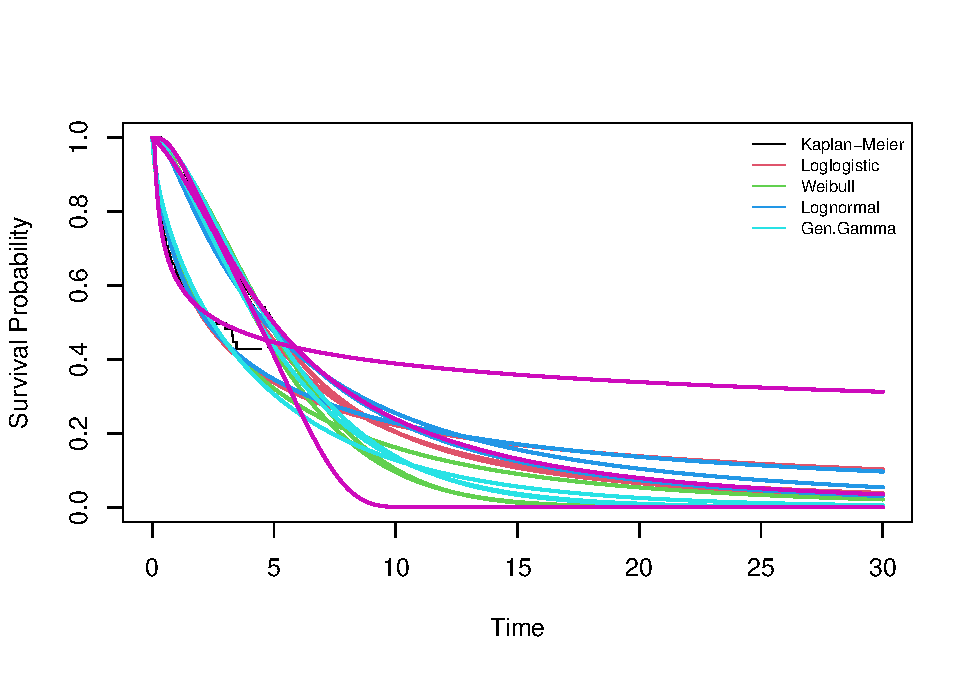
\includegraphics{markov_sick-sicker_PSA_solutions_files/figure-latex/unnamed-chunk-9-1.pdf}

\hypertarget{overall-survival-os}{%
\subsection{06.2 Overall Survival (OS)}\label{overall-survival-os}}

\begin{Shaded}
\begin{Highlighting}[]
\CommentTok{# calculate the overall survival (OS) probability for no treatment}
\NormalTok{v_os_notrt <-}\StringTok{ }\DecValTok{1} \OperatorTok{-}\StringTok{ }\NormalTok{m_M_notrt[, }\StringTok{"D"}\NormalTok{]    }
\CommentTok{# alternative way of calculating the OS probability   }
\NormalTok{v_os_notrt <-}\StringTok{ }\KeywordTok{rowSums}\NormalTok{(m_M_notrt[, }\DecValTok{1}\OperatorTok{:}\DecValTok{3}\NormalTok{])  }
\CommentTok{# create a simple plot showing the OS}
\KeywordTok{plot}\NormalTok{(}\DecValTok{0}\OperatorTok{:}\NormalTok{n_t, v_os_notrt, }\DataTypeTok{type =} \StringTok{'l'}\NormalTok{, }
     \DataTypeTok{ylim =} \KeywordTok{c}\NormalTok{(}\DecValTok{0}\NormalTok{, }\DecValTok{1}\NormalTok{),}
     \DataTypeTok{ylab =} \StringTok{"Survival probability"}\NormalTok{,}
     \DataTypeTok{xlab =} \StringTok{"Cycle"}\NormalTok{,}
     \DataTypeTok{main =} \StringTok{"Overall Survival"}\NormalTok{)          }
\CommentTok{# add grid }
\KeywordTok{grid}\NormalTok{(}\DataTypeTok{nx =}\NormalTok{ n_t, }\DataTypeTok{ny =} \DecValTok{10}\NormalTok{, }\DataTypeTok{col =} \StringTok{"lightgray"}\NormalTok{, }\DataTypeTok{lty =} \StringTok{"dotted"}\NormalTok{, }\DataTypeTok{lwd =} \KeywordTok{par}\NormalTok{(}\StringTok{"lwd"}\NormalTok{), }
     \DataTypeTok{equilogs =} \OtherTok{TRUE}\NormalTok{) }
\end{Highlighting}
\end{Shaded}

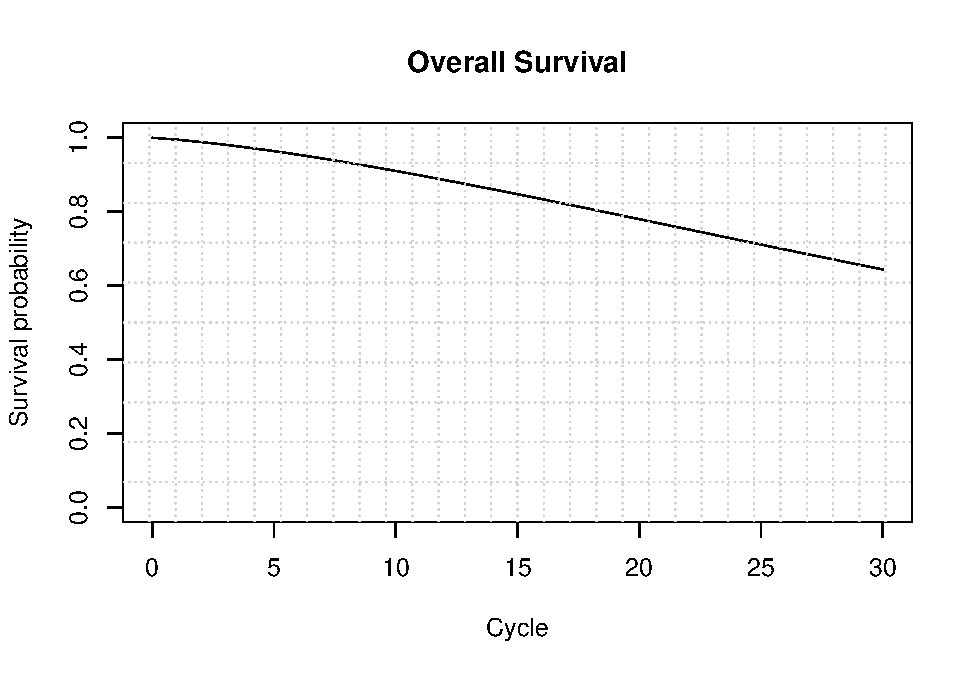
\includegraphics{markov_sick-sicker_PSA_solutions_files/figure-latex/unnamed-chunk-10-1.pdf}

\hypertarget{life-expectancy-le}{%
\subsection{06.2.1 Life Expectancy (LE)}\label{life-expectancy-le}}

\begin{Shaded}
\begin{Highlighting}[]
\NormalTok{v_le <-}\StringTok{ }\KeywordTok{sum}\NormalTok{(v_os_notrt)     }\CommentTok{# summing probablity of OS over time  (i.e. life expectancy)}
\end{Highlighting}
\end{Shaded}

\hypertarget{disease-prevalence}{%
\subsection{06.3 Disease prevalence}\label{disease-prevalence}}

\begin{Shaded}
\begin{Highlighting}[]
\NormalTok{v_prev <-}\StringTok{ }\KeywordTok{rowSums}\NormalTok{(m_M_notrt[, }\KeywordTok{c}\NormalTok{(}\StringTok{"S1"}\NormalTok{, }\StringTok{"S2"}\NormalTok{)]) }\OperatorTok{/}\StringTok{ }\NormalTok{v_os_notrt}
\KeywordTok{plot}\NormalTok{(v_prev,}
     \DataTypeTok{ylim =} \KeywordTok{c}\NormalTok{(}\DecValTok{0}\NormalTok{, }\DecValTok{1}\NormalTok{),}
     \DataTypeTok{ylab =} \StringTok{"Prevalence"}\NormalTok{,}
     \DataTypeTok{xlab =} \StringTok{"Cycle"}\NormalTok{,}
     \DataTypeTok{main =} \StringTok{"Disease prevalence"}\NormalTok{)}
\end{Highlighting}
\end{Shaded}

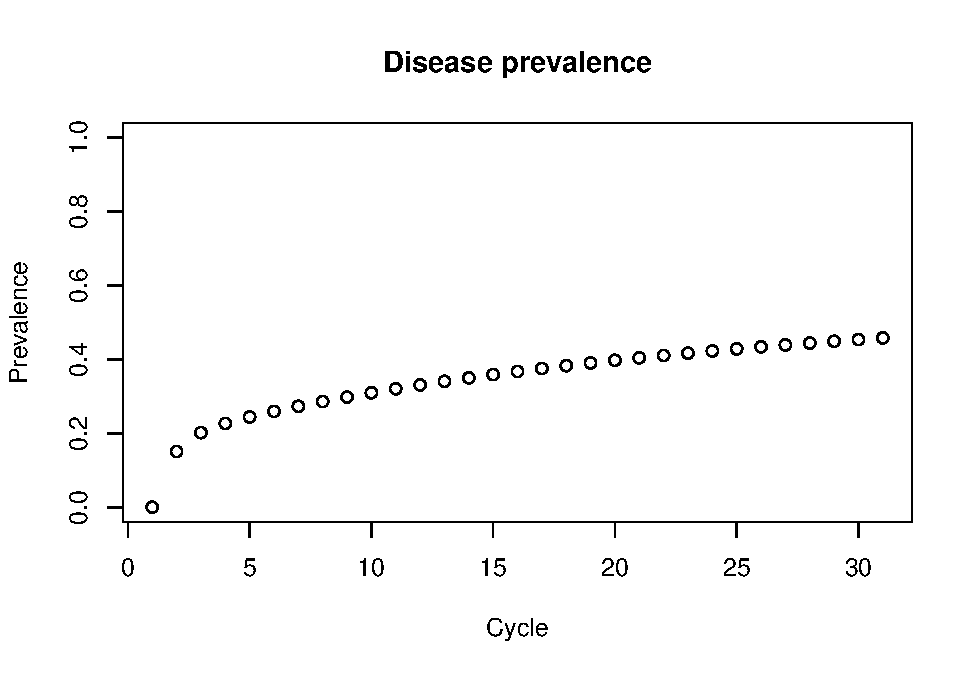
\includegraphics{markov_sick-sicker_PSA_solutions_files/figure-latex/unnamed-chunk-12-1.pdf}

\hypertarget{proportion-of-sick-in-s1-state}{%
\subsection{06.4 Proportion of sick in S1
state}\label{proportion-of-sick-in-s1-state}}

\begin{Shaded}
\begin{Highlighting}[]
\NormalTok{v_prop_S1 <-}\StringTok{ }\NormalTok{m_M_notrt[, }\StringTok{"S1"}\NormalTok{] }\OperatorTok{/}\StringTok{ }\NormalTok{v_prev}
\KeywordTok{plot}\NormalTok{(}\DecValTok{0}\OperatorTok{:}\NormalTok{n_t, v_prop_S1,}
     \DataTypeTok{xlab =} \StringTok{"Cycle"}\NormalTok{, }
     \DataTypeTok{ylab =} \StringTok{"Proportion"}\NormalTok{, }
     \DataTypeTok{main =} \StringTok{"Proportion of sick in S1 state"}\NormalTok{, }
     \DataTypeTok{col  =} \StringTok{"black"}\NormalTok{, }\DataTypeTok{type =} \StringTok{"l"}\NormalTok{)}
\end{Highlighting}
\end{Shaded}

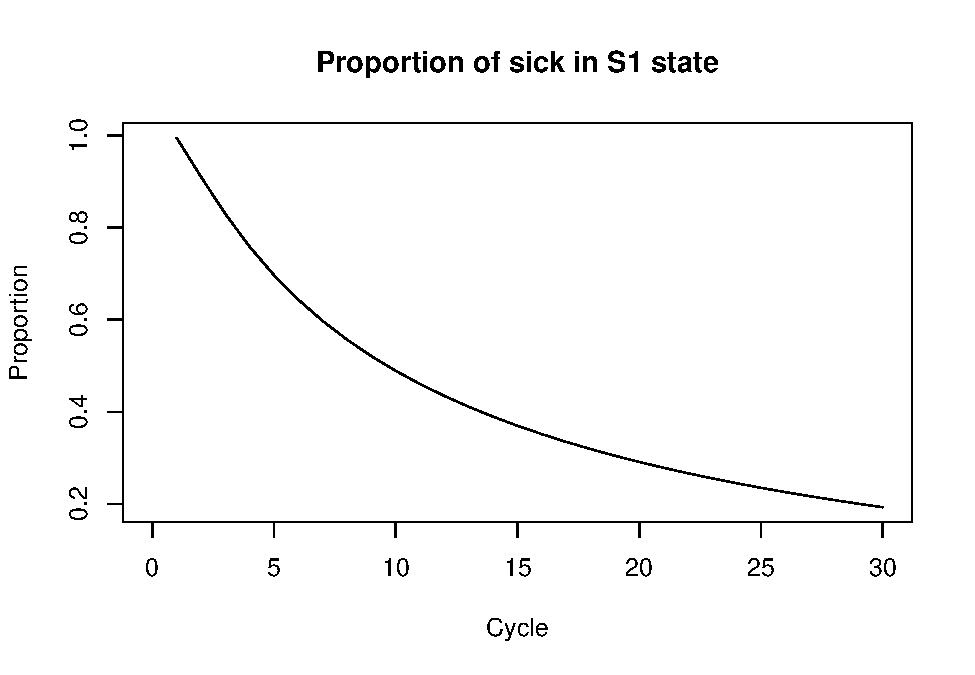
\includegraphics{markov_sick-sicker_PSA_solutions_files/figure-latex/unnamed-chunk-13-1.pdf}

\hypertarget{compute-cost-effectiveness-outcomes}{%
\section{07 Compute Cost-Effectiveness
Outcomes}\label{compute-cost-effectiveness-outcomes}}

\begin{Shaded}
\begin{Highlighting}[]
\CommentTok{# Vectors with costs and utilities by treatment}
\NormalTok{v_u_notrt   <-}\StringTok{ }\KeywordTok{c}\NormalTok{(u_H, u_S1, u_S2, u_D)}
\NormalTok{v_u_trt     <-}\StringTok{ }\KeywordTok{c}\NormalTok{(u_H, u_trt, u_S2, u_D)}

\NormalTok{v_c_notrt   <-}\StringTok{ }\KeywordTok{c}\NormalTok{(c_H, c_S1, c_S2, c_D)}
\NormalTok{v_c_trt     <-}\StringTok{ }\KeywordTok{c}\NormalTok{(c_H, c_S1 }\OperatorTok{+}\StringTok{ }\NormalTok{c_trt, c_S2 }\OperatorTok{+}\StringTok{ }\NormalTok{c_trt, c_D)}
\end{Highlighting}
\end{Shaded}

\hypertarget{mean-costs-and-qalys-for-treatment-and-no-treatment}{%
\subsection{07.1 Mean Costs and QALYs for Treatment and NO
Treatment}\label{mean-costs-and-qalys-for-treatment-and-no-treatment}}

\begin{Shaded}
\begin{Highlighting}[]
\NormalTok{v_tu_notrt  <-}\StringTok{ }\NormalTok{m_M_notrt   }\OperatorTok\StringTok{  }\NormalTok{v_u_notrt}
\NormalTok{v_tu_trt    <-}\StringTok{ }\NormalTok{m_M_trt     }\OperatorTok\StringTok{  }\NormalTok{v_u_trt}

\NormalTok{v_tc_notrt  <-}\StringTok{ }\NormalTok{m_M_notrt   }\OperatorTok\StringTok{  }\NormalTok{v_c_notrt}
\NormalTok{v_tc_trt    <-}\StringTok{ }\NormalTok{m_M_trt     }\OperatorTok\StringTok{  }\NormalTok{v_c_trt }
\end{Highlighting}
\end{Shaded}

\hypertarget{discounted-mean-costs-and-qalys}{%
\subsection{07.2 Discounted Mean Costs and
QALYs}\label{discounted-mean-costs-and-qalys}}

\begin{Shaded}
\begin{Highlighting}[]
\NormalTok{tu_d_notrt  <-}\StringTok{ }\KeywordTok{t}\NormalTok{(v_tu_notrt)   }\OperatorTok\StringTok{  }\NormalTok{v_dwe   }
\NormalTok{tu_d_trt    <-}\StringTok{ }\KeywordTok{t}\NormalTok{(v_tu_trt)     }\OperatorTok\StringTok{  }\NormalTok{v_dwe}

\NormalTok{tc_d_notrt  <-}\StringTok{ }\KeywordTok{t}\NormalTok{(v_tc_notrt)   }\OperatorTok\StringTok{  }\NormalTok{v_dwc}
\NormalTok{tc_d_trt    <-}\StringTok{ }\KeywordTok{t}\NormalTok{(v_tc_trt)     }\OperatorTok\StringTok{  }\NormalTok{v_dwc}

\CommentTok{# store them into a vector}
\NormalTok{v_tc_d      <-}\StringTok{ }\KeywordTok{c}\NormalTok{(tc_d_notrt, tc_d_trt)}
\NormalTok{v_tu_d      <-}\StringTok{ }\KeywordTok{c}\NormalTok{(tu_d_notrt, tu_d_trt)}

\CommentTok{# Dataframe with discounted costs and effectiveness}
\NormalTok{df_ce       <-}\StringTok{ }\KeywordTok{data.frame}\NormalTok{(}\DataTypeTok{Strategy =}\NormalTok{ v_names_str,}
                          \DataTypeTok{Cost     =}\NormalTok{ v_tc_d,}
                          \DataTypeTok{Effect   =}\NormalTok{ v_tu_d)}
\NormalTok{df_ce}
\end{Highlighting}
\end{Shaded}

\begin{verbatim}
##       Strategy      Cost   Effect
## 1 No Treatment  75976.15 15.83885
## 2    Treatment 141623.03 16.40041
\end{verbatim}

\hypertarget{compute-icers-of-the-markov-model}{%
\subsection{07.3 Compute ICERs of the Markov
model}\label{compute-icers-of-the-markov-model}}

\begin{Shaded}
\begin{Highlighting}[]
\NormalTok{df_cea <-}\StringTok{ }\KeywordTok{calculate_icers}\NormalTok{(}\DataTypeTok{cost       =}\NormalTok{ df_ce}\OperatorTok{$}\NormalTok{Cost,}
                          \DataTypeTok{effect     =}\NormalTok{ df_ce}\OperatorTok{$}\NormalTok{Effect,}
                          \DataTypeTok{strategies =}\NormalTok{ df_ce}\OperatorTok{$}\NormalTok{Strategy)}
\NormalTok{df_cea}
\end{Highlighting}
\end{Shaded}

\begin{verbatim}
##       Strategy      Cost   Effect Inc_Cost Inc_Effect     ICER Status
## 1 No Treatment  75976.15 15.83885       NA         NA       NA     ND
## 2    Treatment 141623.03 16.40041 65646.88  0.5615578 116901.4     ND
\end{verbatim}

\hypertarget{plot-frontier-of-the-markov-model}{%
\subsection{07.4 Plot frontier of the Markov
model}\label{plot-frontier-of-the-markov-model}}

\begin{Shaded}
\begin{Highlighting}[]
\KeywordTok{plot}\NormalTok{(df_cea, }\DataTypeTok{effect_units =} \StringTok{"Quality of Life"}\NormalTok{, }\DataTypeTok{xlim =} \KeywordTok{c}\NormalTok{(}\FloatTok{15.6}\NormalTok{, }\FloatTok{16.6}\NormalTok{))}
\end{Highlighting}
\end{Shaded}

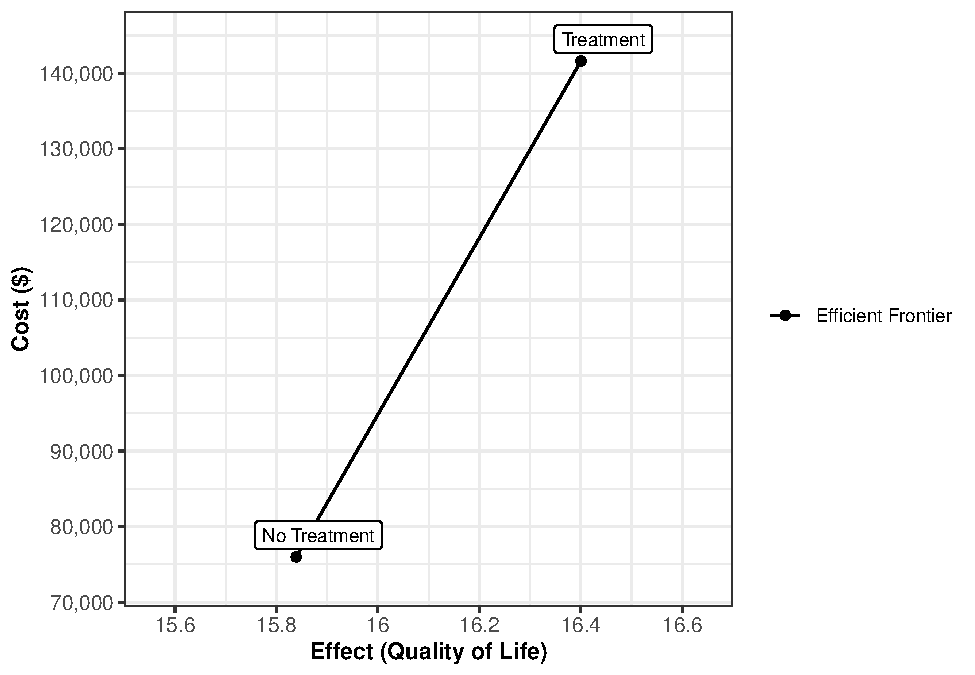
\includegraphics{markov_sick-sicker_PSA_solutions_files/figure-latex/unnamed-chunk-18-1.pdf}

\hypertarget{deterministic-sensitivity-analysis}{%
\section{08 Deterministic Sensitivity
Analysis}\label{deterministic-sensitivity-analysis}}

\hypertarget{list-of-input-parameters}{%
\subsection{08.1 List of input
parameters}\label{list-of-input-parameters}}

Create list \texttt{l\_params\_all} with all input probabilities, cost
and utilities.

\begin{Shaded}
\begin{Highlighting}[]
\NormalTok{l_params_all <-}\StringTok{ }\KeywordTok{list}\NormalTok{(}
  \DataTypeTok{p_HD    =} \FloatTok{0.005}\NormalTok{,  }\CommentTok{# probability to die when healthy}
  \DataTypeTok{p_HS1   =} \FloatTok{0.15}\NormalTok{,   }\CommentTok{# probability to become sick when healthy}
  \DataTypeTok{p_S1H   =} \FloatTok{0.5}\NormalTok{,    }\CommentTok{# probability to become healthy when sick}
  \DataTypeTok{p_S1S2  =} \FloatTok{0.105}\NormalTok{,  }\CommentTok{# probability to become sicker when sick}
  \DataTypeTok{hr_S1   =} \DecValTok{3}\NormalTok{,      }\CommentTok{# hazard ratio of death in sick vs healthy}
  \DataTypeTok{hr_S2   =} \DecValTok{10}\NormalTok{,     }\CommentTok{# hazard ratio of death in sicker vs healthy}
  \DataTypeTok{c_H     =} \DecValTok{2000}\NormalTok{,   }\CommentTok{# cost of remaining one cycle in the healthy state}
  \DataTypeTok{c_S1    =} \DecValTok{4000}\NormalTok{,   }\CommentTok{# cost of remaining one cycle in the sick state}
  \DataTypeTok{c_S2    =} \DecValTok{15000}\NormalTok{,  }\CommentTok{# cost of remaining one cycle in the sicker state}
  \DataTypeTok{c_trt   =} \DecValTok{12000}\NormalTok{,  }\CommentTok{# cost of treatment(per cycle)}
  \DataTypeTok{c_D     =} \DecValTok{0}\NormalTok{,      }\CommentTok{# cost of being in the death state}
  \DataTypeTok{u_H     =} \DecValTok{1}\NormalTok{,      }\CommentTok{# utility when healthy}
  \DataTypeTok{u_S1    =} \FloatTok{0.75}\NormalTok{,   }\CommentTok{# utility when sick}
  \DataTypeTok{u_S2    =} \FloatTok{0.5}\NormalTok{,    }\CommentTok{# utility when sicker}
  \DataTypeTok{u_D     =} \DecValTok{0}\NormalTok{,      }\CommentTok{# utility when dead}
  \DataTypeTok{u_trt   =} \FloatTok{0.95}\NormalTok{,   }\CommentTok{# utility when treated}
  \DataTypeTok{d_e     =} \FloatTok{0.03}\NormalTok{,   }\CommentTok{# discount factor for effectiveness}
  \DataTypeTok{d_c     =} \FloatTok{0.03}    \CommentTok{# discount factor for costs}
\NormalTok{)}

\CommentTok{# store the parameter names into a vector}
\NormalTok{v_names_parms <-}\StringTok{ }\KeywordTok{names}\NormalTok{(l_params_all)}
\end{Highlighting}
\end{Shaded}

\hypertarget{load-sick-sicker-markov-model-function}{%
\subsection{08.2 Load Sick-Sicker Markov model
function}\label{load-sick-sicker-markov-model-function}}

\begin{Shaded}
\begin{Highlighting}[]
\KeywordTok{source}\NormalTok{(}\StringTok{"Functions_markov_sick-sicker.R"}\NormalTok{)}
\CommentTok{# Test function}
\KeywordTok{calculate_ce_out}\NormalTok{(l_params_all)}
\end{Highlighting}
\end{Shaded}

\begin{verbatim}
##       Strategy      Cost   Effect     NMB
## 1 No Treatment  75976.15 15.83885 1507909
## 2    Treatment 141623.03 16.40041 1498418
\end{verbatim}

\hypertarget{one-way-sensitivity-analysis-owsa}{%
\subsection{08.3 One-way sensitivity analysis
(OWSA)}\label{one-way-sensitivity-analysis-owsa}}

\begin{Shaded}
\begin{Highlighting}[]
\KeywordTok{options}\NormalTok{(}\DataTypeTok{scipen =} \DecValTok{999}\NormalTok{) }\CommentTok{# disabling scientific notation in R}
\CommentTok{# dataframe containing all parameters, their basecase values, and the min and }
\CommentTok{# max values of the parameters of interest }
\NormalTok{df_params_owsa <-}\StringTok{ }\KeywordTok{data.frame}\NormalTok{(}\DataTypeTok{pars =} \KeywordTok{c}\NormalTok{(}\StringTok{"p_S1S2"}\NormalTok{, }\StringTok{"c_trt"}\NormalTok{, }\StringTok{"u_S1"}\NormalTok{, }\StringTok{"u_trt"}\NormalTok{),}
                             \DataTypeTok{min  =} \KeywordTok{c}\NormalTok{(}\FloatTok{0.05}\NormalTok{ ,  }\DecValTok{6000}\NormalTok{ , }\FloatTok{0.65}\NormalTok{, }\FloatTok{0.80}\NormalTok{), }\CommentTok{# min parameter values}
                             \DataTypeTok{max  =} \KeywordTok{c}\NormalTok{(}\FloatTok{0.155}\NormalTok{, }\DecValTok{18000}\NormalTok{ , }\FloatTok{0.85}\NormalTok{, }\FloatTok{0.98}\NormalTok{)  }\CommentTok{# max parameter values}
\NormalTok{                             )}

\NormalTok{owsa_nmb  <-}\StringTok{ }\KeywordTok{run_owsa_det}\NormalTok{(}\DataTypeTok{params_range     =}\NormalTok{ df_params_owsa,   }\CommentTok{# dataframe with parameters for owsa}
                          \DataTypeTok{params_basecase  =}\NormalTok{ l_params_all,     }\CommentTok{# list with all parameters}
                          \DataTypeTok{nsamp            =} \DecValTok{100}\NormalTok{,              }\CommentTok{# number of parameter values}
                          \DataTypeTok{FUN              =}\NormalTok{ calculate_ce_out, }\CommentTok{# function to compute outputs}
                          \DataTypeTok{outcomes         =} \KeywordTok{c}\NormalTok{(}\StringTok{"NMB"}\NormalTok{),         }\CommentTok{# output to do the OWSA on}
                          \DataTypeTok{strategies       =}\NormalTok{ v_names_str,      }\CommentTok{# names of the strategies}
                          \DataTypeTok{n_wtp            =} \DecValTok{120000}\NormalTok{)           }\CommentTok{# extra argument to pass to FUN}
\end{Highlighting}
\end{Shaded}

\begin{verbatim}
## Warning: strategy name 'No Treatment' was converted to 'No.Treatment' for
## compatibility. See ?make.names
\end{verbatim}

\hypertarget{plot-owsa}{%
\subsection{08.3.1 Plot OWSA}\label{plot-owsa}}

\begin{Shaded}
\begin{Highlighting}[]
\KeywordTok{plot}\NormalTok{(owsa_nmb, }\DataTypeTok{txtsize =} \DecValTok{16}\NormalTok{, }\DataTypeTok{n_x_ticks =} \DecValTok{5}\NormalTok{, }\DataTypeTok{n_y_ticks =} \DecValTok{3}\NormalTok{,}
     \DataTypeTok{facet_scales =} \StringTok{"free"}\NormalTok{) }\OperatorTok{+}
\StringTok{     }\KeywordTok{theme}\NormalTok{(}\DataTypeTok{legend.position =} \StringTok{"bottom"}\NormalTok{, }
           \DataTypeTok{axis.text.x =} \KeywordTok{element_text}\NormalTok{(}\DataTypeTok{angle =} \DecValTok{45}\NormalTok{, }\DataTypeTok{vjust =} \FloatTok{0.5}\NormalTok{))}
\end{Highlighting}
\end{Shaded}

\includegraphics{markov_sick-sicker_PSA_solutions_files/figure-latex/unnamed-chunk-22-1.pdf}

\hypertarget{optimal-strategy-with-owsa}{%
\subsection{08.3.2 Optimal strategy with
OWSA}\label{optimal-strategy-with-owsa}}

\begin{Shaded}
\begin{Highlighting}[]
\KeywordTok{owsa_opt_strat}\NormalTok{(}\DataTypeTok{owsa =}\NormalTok{ owsa_nmb)}
\end{Highlighting}
\end{Shaded}

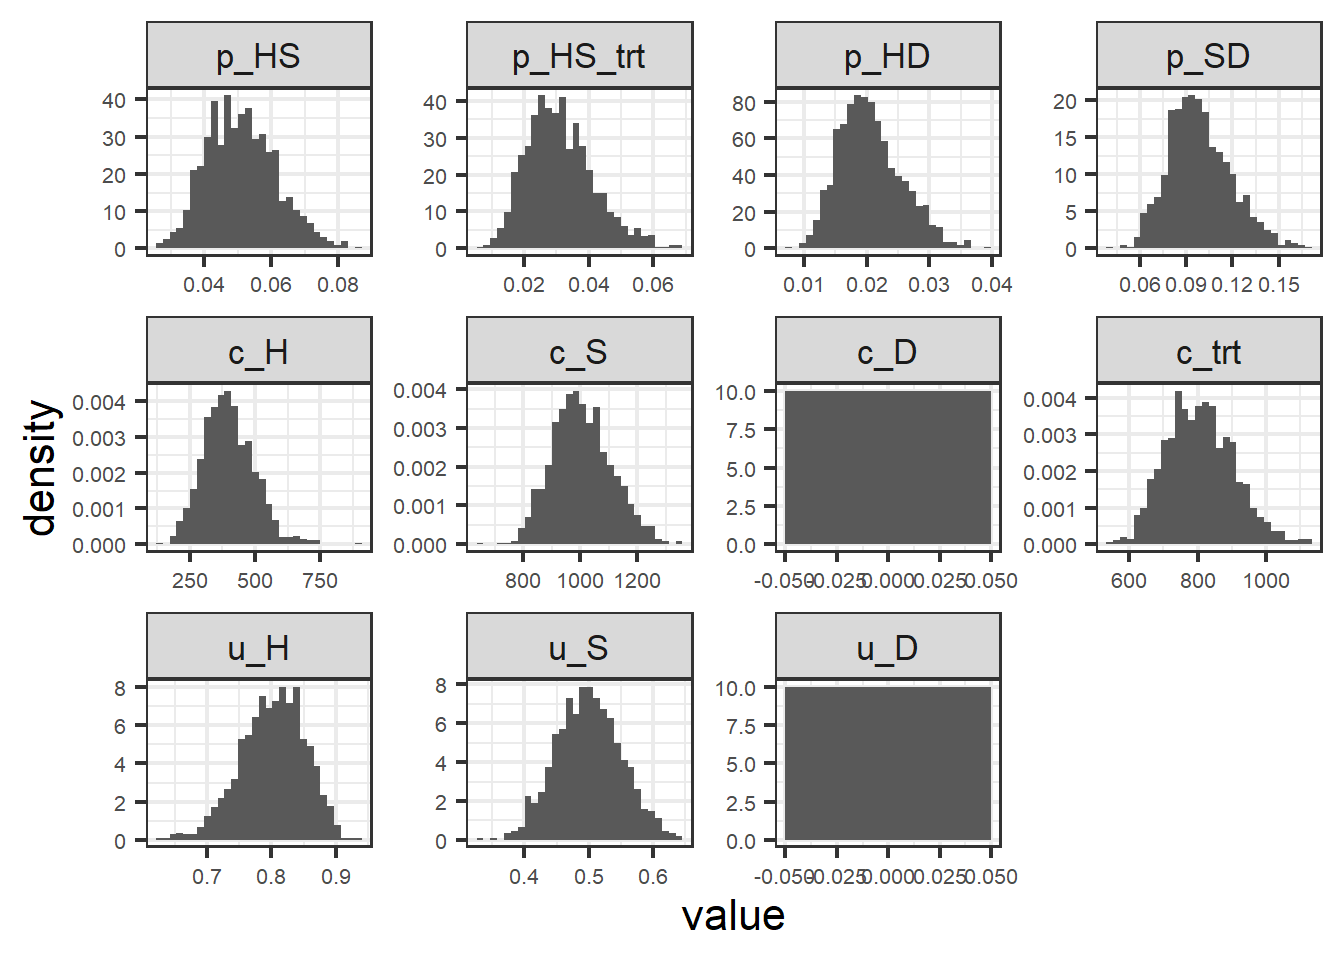
\includegraphics{markov_sick-sicker_PSA_solutions_files/figure-latex/unnamed-chunk-23-1.pdf}

\hypertarget{tornado-plot}{%
\subsection{08.3.3 Tornado plot}\label{tornado-plot}}

\begin{Shaded}
\begin{Highlighting}[]
\KeywordTok{owsa_tornado}\NormalTok{(}\DataTypeTok{owsa =}\NormalTok{ owsa_nmb)}
\end{Highlighting}
\end{Shaded}

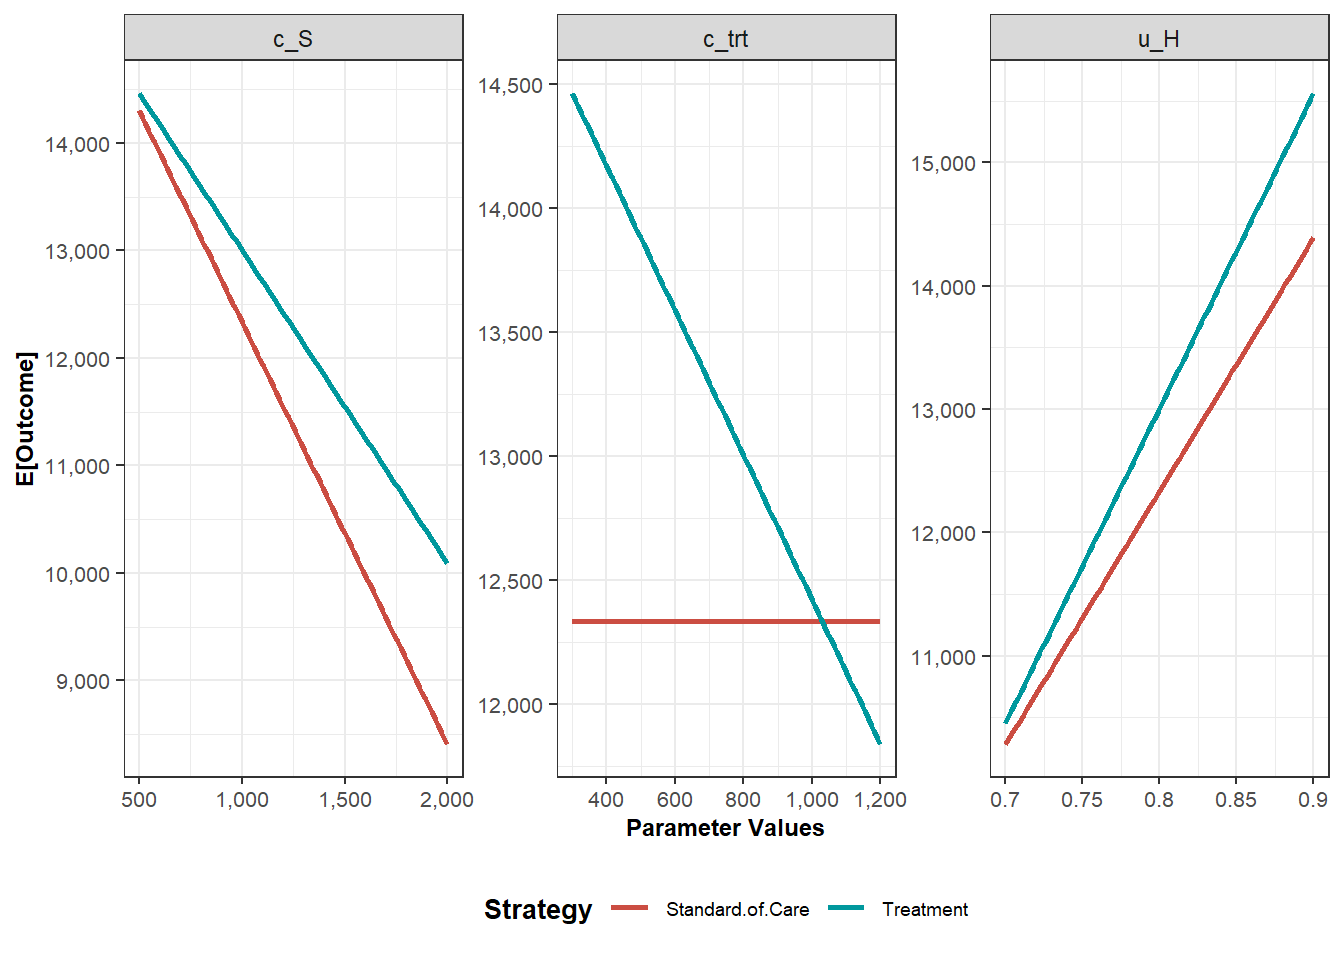
\includegraphics{markov_sick-sicker_PSA_solutions_files/figure-latex/unnamed-chunk-24-1.pdf}

\hypertarget{two-way-sensitivity-analysis-twsa}{%
\subsection{08.4 Two-way sensitivity analysis
(TWSA)}\label{two-way-sensitivity-analysis-twsa}}

\begin{Shaded}
\begin{Highlighting}[]
\CommentTok{# dataframe containing all parameters, their basecase values, and the min and }
\CommentTok{# max values of the parameters of interest}
\NormalTok{df_params_twsa <-}\StringTok{ }\KeywordTok{data.frame}\NormalTok{(}\DataTypeTok{pars =} \KeywordTok{c}\NormalTok{(}\StringTok{"c_trt"}\NormalTok{, }\StringTok{"u_trt"}\NormalTok{),}
                             \DataTypeTok{min  =} \KeywordTok{c}\NormalTok{(}\DecValTok{6000}\NormalTok{, }\FloatTok{0.80}\NormalTok{), }\CommentTok{# min parameter values}
                             \DataTypeTok{max  =} \KeywordTok{c}\NormalTok{(}\DecValTok{18000}\NormalTok{, }\FloatTok{0.98}\NormalTok{) }\CommentTok{# max parameter values}
\NormalTok{                             )}

\NormalTok{twsa_nmb <-}\StringTok{ }\KeywordTok{run_twsa_det}\NormalTok{(}\DataTypeTok{params_range    =}\NormalTok{ df_params_twsa,   }\CommentTok{# dataframe with parameters for twsa}
                         \DataTypeTok{params_basecase =}\NormalTok{ l_params_all,     }\CommentTok{# list with all parameters}
                         \DataTypeTok{nsamp           =} \DecValTok{40}\NormalTok{,               }\CommentTok{# number of parameter values}
                         \DataTypeTok{FUN             =}\NormalTok{ calculate_ce_out, }\CommentTok{# function to compute outputs}
                         \DataTypeTok{outcomes        =} \KeywordTok{c}\NormalTok{(}\StringTok{"NMB"}\NormalTok{),         }\CommentTok{# output to do the twsa on}
                         \DataTypeTok{strategies      =}\NormalTok{ v_names_str,      }\CommentTok{# names of the strategies}
                         \DataTypeTok{n_wtp           =} \DecValTok{120000}\NormalTok{)           }\CommentTok{# extra argument to pass to FUN}
\end{Highlighting}
\end{Shaded}

\hypertarget{plot-twsa}{%
\subsection{08.4.1 Plot TWSA}\label{plot-twsa}}

\begin{Shaded}
\begin{Highlighting}[]
\KeywordTok{plot}\NormalTok{(twsa_nmb) }\OperatorTok{+}\StringTok{ }
\StringTok{  }\KeywordTok{ggtitle}\NormalTok{(}\DataTypeTok{label =} \StringTok{"Two-way sensitivity analysis"}\NormalTok{, }
          \DataTypeTok{subtitle =} \StringTok{"Net monetary benefit"}\NormalTok{) }\OperatorTok{+}
\StringTok{          }\KeywordTok{theme}\NormalTok{(}\DataTypeTok{legend.position =} \StringTok{"bottom"}\NormalTok{)}
\end{Highlighting}
\end{Shaded}

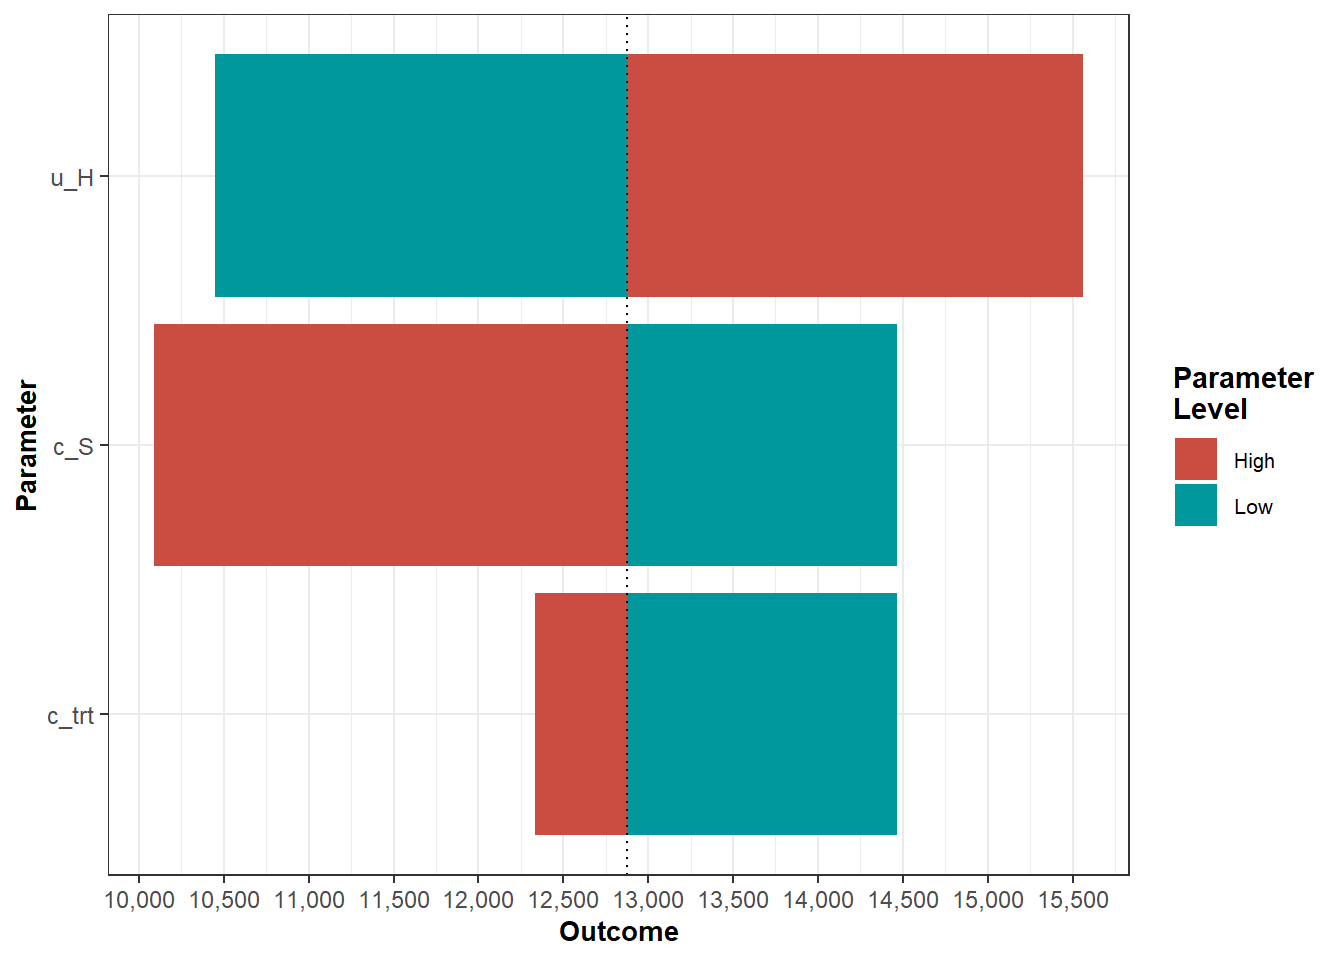
\includegraphics{markov_sick-sicker_PSA_solutions_files/figure-latex/unnamed-chunk-26-1.pdf}

\hypertarget{probabilistic-sensitivity-analysis-psa}{%
\section{09 Probabilistic Sensitivity Analysis
(PSA)}\label{probabilistic-sensitivity-analysis-psa}}

\begin{Shaded}
\begin{Highlighting}[]
\CommentTok{# Function to generate PSA input dataset}
\NormalTok{generate_psa_params <-}\StringTok{ }\ControlFlowTok{function}\NormalTok{(}\DataTypeTok{n_sim =} \DecValTok{1000}\NormalTok{, }\DataTypeTok{seed =} \DecValTok{071818}\NormalTok{)\{}
  \KeywordTok{set.seed}\NormalTok{(seed) }\CommentTok{# set a seed to be able to reproduce the same results}
\NormalTok{  df_psa <-}\StringTok{ }\KeywordTok{data.frame}\NormalTok{(}
    \CommentTok{# Transition probabilities (per cycle)}
    \DataTypeTok{p_HS1   =} \KeywordTok{rbeta}\NormalTok{(n_sim, }\DecValTok{30}\NormalTok{, }\DecValTok{170}\NormalTok{) , }\CommentTok{# probability to become sick when healthy}
    \DataTypeTok{p_S1H   =} \KeywordTok{rbeta}\NormalTok{(n_sim, }\DecValTok{60}\NormalTok{, }\DecValTok{60}\NormalTok{)  , }\CommentTok{# probability to become healthy when sick}
    \DataTypeTok{p_S1S2  =} \KeywordTok{rbeta}\NormalTok{(n_sim, }\DecValTok{84}\NormalTok{, }\DecValTok{716}\NormalTok{) , }\CommentTok{# probability to become sicker when sick}
    \DataTypeTok{p_HD    =} \KeywordTok{rbeta}\NormalTok{(n_sim, }\DecValTok{10}\NormalTok{, }\DecValTok{1990}\NormalTok{), }\CommentTok{# probability to die when healthy}
    \DataTypeTok{hr_S1   =} \KeywordTok{rlnorm}\NormalTok{(n_sim, }\KeywordTok{log}\NormalTok{(}\DecValTok{3}\NormalTok{),  }\FloatTok{0.01}\NormalTok{), }\CommentTok{# rate ratio of death in S1 vs healthy}
    \DataTypeTok{hr_S2   =} \KeywordTok{rlnorm}\NormalTok{(n_sim, }\KeywordTok{log}\NormalTok{(}\DecValTok{10}\NormalTok{), }\FloatTok{0.02}\NormalTok{), }\CommentTok{# rate ratio of death in S2 vs healthy }
    
    \CommentTok{# State rewards}
    \CommentTok{# Costs}
    \DataTypeTok{c_H   =} \KeywordTok{rgamma}\NormalTok{(n_sim, }\DataTypeTok{shape =} \DecValTok{100}\NormalTok{, }\DataTypeTok{scale =} \DecValTok{20}\NormalTok{)    , }\CommentTok{# cost of remaining one cycle in state H}
    \DataTypeTok{c_S1  =} \KeywordTok{rgamma}\NormalTok{(n_sim, }\DataTypeTok{shape =} \FloatTok{177.8}\NormalTok{, }\DataTypeTok{scale =} \FloatTok{22.5}\NormalTok{), }\CommentTok{# cost of remaining one cycle in state S1}
    \DataTypeTok{c_S2  =} \KeywordTok{rgamma}\NormalTok{(n_sim, }\DataTypeTok{shape =} \DecValTok{225}\NormalTok{, }\DataTypeTok{scale =} \FloatTok{66.7}\NormalTok{)  , }\CommentTok{# cost of remaining one cycle in state S2}
    \DataTypeTok{c_Trt =} \KeywordTok{rgamma}\NormalTok{(n_sim, }\DataTypeTok{shape =} \FloatTok{73.5}\NormalTok{, }\DataTypeTok{scale =} \FloatTok{163.3}\NormalTok{), }\CommentTok{# cost of treatment (per cycle)}
    \DataTypeTok{c_D   =} \DecValTok{0}\NormalTok{                                         , }\CommentTok{# cost of being in the death state}
    
    \CommentTok{# Utilities}
    \DataTypeTok{u_H   =} \KeywordTok{rbeta}\NormalTok{(n_sim, }\DataTypeTok{shape1 =} \DecValTok{200}\NormalTok{, }\DataTypeTok{shape2 =} \DecValTok{3}\NormalTok{)  , }\CommentTok{# utility when healthy}
    \DataTypeTok{u_S1  =} \KeywordTok{rbeta}\NormalTok{(n_sim, }\DataTypeTok{shape1 =} \DecValTok{130}\NormalTok{, }\DataTypeTok{shape2 =} \DecValTok{45}\NormalTok{) , }\CommentTok{# utility when sick}
    \DataTypeTok{u_S2  =} \KeywordTok{rbeta}\NormalTok{(n_sim, }\DataTypeTok{shape1 =} \DecValTok{230}\NormalTok{, }\DataTypeTok{shape2 =} \DecValTok{230}\NormalTok{), }\CommentTok{# utility when sicker}
    \DataTypeTok{u_D   =} \DecValTok{0}\NormalTok{                                       , }\CommentTok{# utility when dead}
    \DataTypeTok{u_Trt =} \KeywordTok{rbeta}\NormalTok{(n_sim, }\DataTypeTok{shape1 =} \DecValTok{300}\NormalTok{, }\DataTypeTok{shape2 =} \DecValTok{15}\NormalTok{) , }\CommentTok{# utility when being treated}
    \DataTypeTok{d_e   =} \FloatTok{0.03}\NormalTok{,  }\CommentTok{# discount factor for effectiveness}
    \DataTypeTok{d_c   =} \FloatTok{0.03}   \CommentTok{# discount factor for costs}
\NormalTok{  )}
    \KeywordTok{return}\NormalTok{(df_psa)}
\NormalTok{\}}
\CommentTok{# Try it}
\KeywordTok{generate_psa_params}\NormalTok{(}\DecValTok{10}\NormalTok{) }
\end{Highlighting}
\end{Shaded}

\begin{verbatim}
##         p_HS1     p_S1H     p_S1S2        p_HD    hr_S1     hr_S2      c_H
## 1  0.15132349 0.4820445 0.08485456 0.003973762 3.055410 10.148768 1887.449
## 2  0.12522484 0.4392546 0.11683397 0.004813328 3.005252  9.928044 1966.291
## 3  0.15673720 0.5311020 0.11925841 0.004491843 2.982392 10.021998 2101.059
## 4  0.11276858 0.4493088 0.09393848 0.010646056 2.981918 10.167486 1728.664
## 5  0.14292946 0.5825087 0.11628065 0.007045338 3.024975 10.006505 2160.895
## 6  0.20088601 0.4580278 0.10403415 0.004058637 2.971345 10.012715 1969.304
## 7  0.14347796 0.5492245 0.09294048 0.005658464 2.989181 10.001860 1641.192
## 8  0.13149270 0.4899896 0.12838861 0.007354969 2.984080  9.919332 2276.032
## 9  0.15593267 0.5705602 0.09237907 0.004162148 2.988974 10.142331 1717.867
## 10 0.09824029 0.5127637 0.10683148 0.002141140 2.968692  9.749869 2132.549
##        c_S1     c_S2    c_Trt c_D       u_H      u_S1      u_S2 u_D     u_Trt
## 1  4173.600 14607.88 10673.74   0 0.9829120 0.7252701 0.4757751   0 0.9435773
## 2  4188.264 14714.84 13380.61   0 0.9693926 0.7610392 0.4591563   0 0.9501528
## 3  4578.682 16664.54 12522.58   0 0.9910033 0.7076433 0.5032719   0 0.9670124
## 4  3395.922 15669.87 13833.65   0 0.9928844 0.7124119 0.5132492   0 0.9649128
## 5  3878.562 15302.70 13154.65   0 0.9748972 0.7344718 0.4895693   0 0.9325969
## 6  3970.522 15303.55 13914.95   0 0.9832065 0.7169406 0.4628316   0 0.9456881
## 7  3680.588 15378.20 12117.86   0 0.9917677 0.7851270 0.4504530   0 0.9093339
## 8  3781.956 15614.73 12070.99   0 0.9727485 0.7582961 0.4727426   0 0.9390084
## 9  3448.146 15401.50 11760.17   0 0.9836544 0.7648816 0.4851046   0 0.9537789
## 10 4656.666 15198.97 10216.98   0 0.9915345 0.7751203 0.5311969   0 0.9577708
##     d_e  d_c
## 1  0.03 0.03
## 2  0.03 0.03
## 3  0.03 0.03
## 4  0.03 0.03
## 5  0.03 0.03
## 6  0.03 0.03
## 7  0.03 0.03
## 8  0.03 0.03
## 9  0.03 0.03
## 10 0.03 0.03
\end{verbatim}

\begin{Shaded}
\begin{Highlighting}[]
\CommentTok{# Number of simulations}
\NormalTok{n_sim <-}\StringTok{ }\DecValTok{1000}

\CommentTok{# Generate PSA input dataset}
\NormalTok{df_psa_input <-}\StringTok{ }\KeywordTok{generate_psa_params}\NormalTok{(}\DataTypeTok{n_sim =}\NormalTok{ n_sim)}
\CommentTok{# First six observations}
\KeywordTok{head}\NormalTok{(df_psa_input)}
\end{Highlighting}
\end{Shaded}

\begin{verbatim}
##       p_HS1     p_S1H    p_S1S2        p_HD    hr_S1     hr_S2      c_H
## 1 0.1513235 0.5617628 0.1033817 0.006269864 2.962948  9.820157 1658.447
## 2 0.1252248 0.4380343 0.1152594 0.005371105 3.014068 10.100813 2050.281
## 3 0.1567372 0.5458102 0.1274505 0.004301015 3.018588  9.825985 2094.425
## 4 0.1127686 0.5106953 0.1015742 0.005319105 2.979709  9.697122 2135.411
## 5 0.1429295 0.5277308 0.1020384 0.004225209 3.025490 10.254387 1665.257
## 6 0.2008860 0.5252364 0.1030676 0.008319206 2.979175 10.366400 2049.794
##       c_S1     c_S2     c_Trt c_D       u_H      u_S1      u_S2 u_D     u_Trt
## 1 4191.109 15165.80 10292.050   0 0.9816602 0.7395884 0.5106656   0 0.9496993
## 2 4133.823 15042.66 10779.006   0 0.9906084 0.7240259 0.4927761   0 0.9731185
## 3 3567.033 15052.49 12811.443   0 0.9834960 0.6910869 0.5024542   0 0.9598494
## 4 3726.226 16084.60 10072.741   0 0.9919197 0.7065183 0.5118351   0 0.9357411
## 5 3654.486 15201.84 14917.228   0 0.9953850 0.6838064 0.5021483   0 0.9635901
## 6 3927.001 17060.57  9581.097   0 0.9813330 0.7766346 0.5035428   0 0.9506926
##    d_e  d_c
## 1 0.03 0.03
## 2 0.03 0.03
## 3 0.03 0.03
## 4 0.03 0.03
## 5 0.03 0.03
## 6 0.03 0.03
\end{verbatim}

\begin{Shaded}
\begin{Highlighting}[]
\CommentTok{# Histogram of parameters}
\KeywordTok{ggplot}\NormalTok{(reshape2}\OperatorTok{::}\KeywordTok{melt}\NormalTok{(df_psa_input, }\DataTypeTok{variable.name =} \StringTok{"Parameter"}\NormalTok{, }
                      \DataTypeTok{value.name =} \StringTok{"Parameter value"}\NormalTok{), }
                      \KeywordTok{aes}\NormalTok{(}\DataTypeTok{x =} \StringTok{`}\DataTypeTok{Parameter value}\StringTok{`}\NormalTok{)) }\OperatorTok{+}
\StringTok{                      }\KeywordTok{facet_wrap}\NormalTok{(}\OperatorTok{~}\NormalTok{Parameter, }\DataTypeTok{scales =} \StringTok{"free"}\NormalTok{) }\OperatorTok{+}
\StringTok{                      }\KeywordTok{geom_histogram}\NormalTok{(}\KeywordTok{aes}\NormalTok{(}\DataTypeTok{y =}\NormalTok{ ..density..), }\DataTypeTok{alpha =} \FloatTok{0.8}\NormalTok{) }\OperatorTok{+}
\StringTok{                      }\KeywordTok{scale_x_continuous}\NormalTok{(}\DataTypeTok{breaks =} \KeywordTok{number_ticks}\NormalTok{(}\DecValTok{2}\NormalTok{)) }\OperatorTok{+}
\StringTok{                      }\KeywordTok{ylab}\NormalTok{(}\StringTok{""}\NormalTok{) }\OperatorTok{+}
\StringTok{                      }\KeywordTok{theme_bw}\NormalTok{(}\DataTypeTok{base_size =} \DecValTok{14}\NormalTok{) }\OperatorTok{+}
\StringTok{                      }\KeywordTok{theme}\NormalTok{(}\DataTypeTok{axis.text.y =} \KeywordTok{element_blank}\NormalTok{(), }\DataTypeTok{text =} \KeywordTok{element_text}\NormalTok{(}\DataTypeTok{size=}\DecValTok{10}\NormalTok{))}
\end{Highlighting}
\end{Shaded}

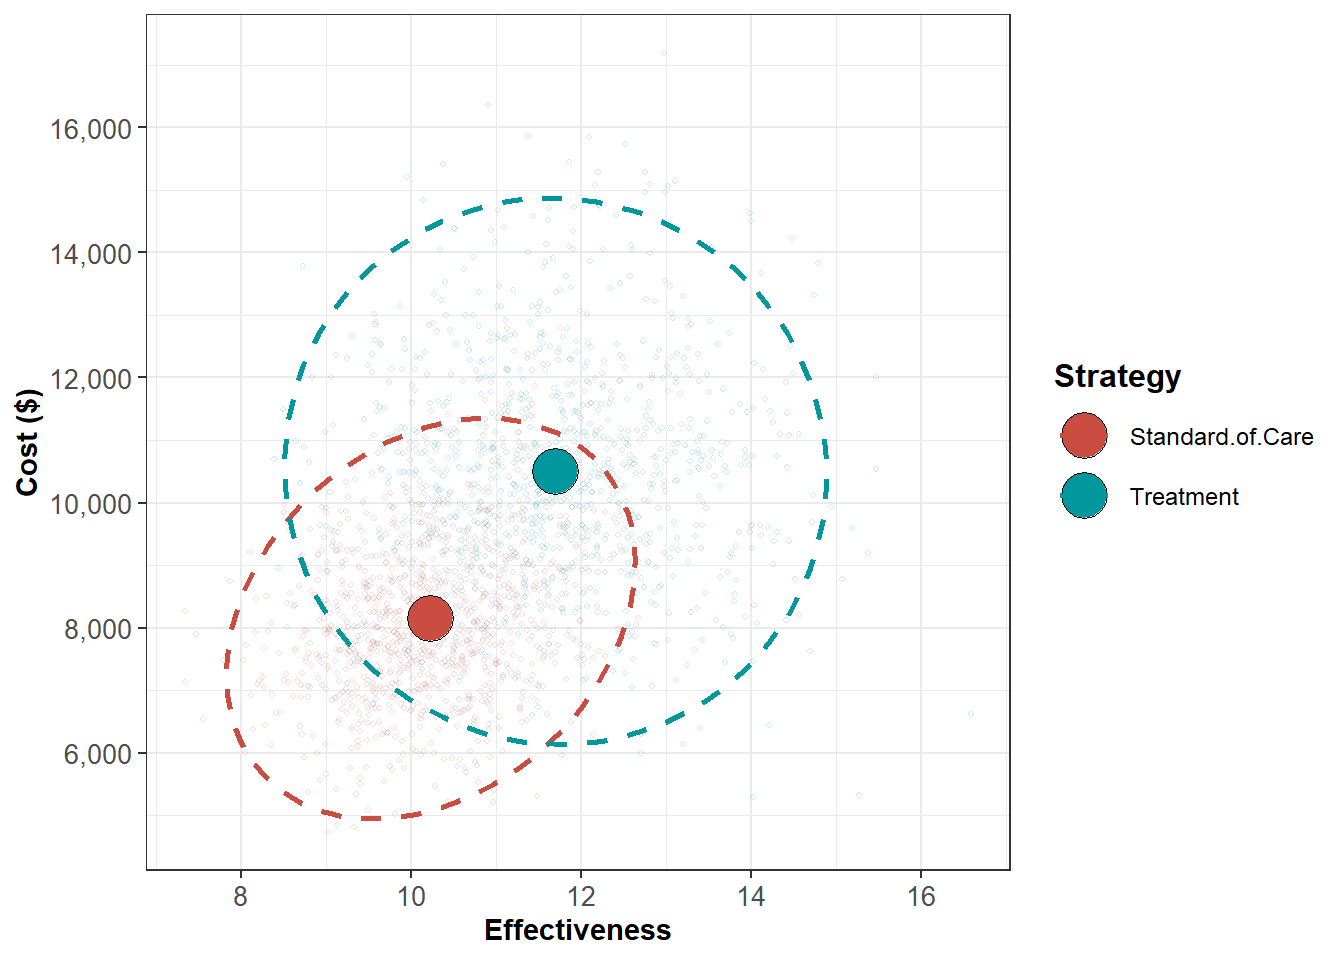
\includegraphics{markov_sick-sicker_PSA_solutions_files/figure-latex/unnamed-chunk-28-1.pdf}

\begin{Shaded}
\begin{Highlighting}[]
\CommentTok{# Initialize dataframes with PSA output }
\CommentTok{# Dataframe of costs}
\NormalTok{df_c <-}\StringTok{ }\KeywordTok{as.data.frame}\NormalTok{(}\KeywordTok{matrix}\NormalTok{(}\DecValTok{0}\NormalTok{, }
                      \DataTypeTok{nrow =}\NormalTok{ n_sim,}
                      \DataTypeTok{ncol =}\NormalTok{ n_str))}
\KeywordTok{colnames}\NormalTok{(df_c) <-}\StringTok{ }\NormalTok{v_names_str}
\CommentTok{# Dataframe of effectiveness}
\NormalTok{df_e <-}\StringTok{ }\KeywordTok{as.data.frame}\NormalTok{(}\KeywordTok{matrix}\NormalTok{(}\DecValTok{0}\NormalTok{, }
                      \DataTypeTok{nrow =}\NormalTok{ n_sim,}
                      \DataTypeTok{ncol =}\NormalTok{ n_str))}
\KeywordTok{colnames}\NormalTok{(df_e) <-}\StringTok{ }\NormalTok{v_names_str}
\end{Highlighting}
\end{Shaded}

\hypertarget{conduct-probabilistic-sensitivity-analysis}{%
\subsection{09.1 Conduct probabilistic sensitivity
analysis}\label{conduct-probabilistic-sensitivity-analysis}}

\begin{Shaded}
\begin{Highlighting}[]
\CommentTok{# Run Markov model on each parameter set of PSA input dataset}
\ControlFlowTok{for}\NormalTok{(i }\ControlFlowTok{in} \DecValTok{1}\OperatorTok{:}\NormalTok{n_sim)\{}
\NormalTok{  l_psa_input <-}\StringTok{ }\KeywordTok{update_param_list}\NormalTok{(l_params_all, df_psa_input[i,])}
\NormalTok{  df_out_psa  <-}\StringTok{ }\KeywordTok{calculate_ce_out}\NormalTok{(l_psa_input)}
\NormalTok{  df_c[i, ] <-}\StringTok{ }\NormalTok{df_out_psa}\OperatorTok{$}\NormalTok{Cost}
\NormalTok{  df_e[i, ] <-}\StringTok{ }\NormalTok{df_out_psa}\OperatorTok{$}\NormalTok{Effect}
  \CommentTok{# Display simulation progress}
  \ControlFlowTok{if}\NormalTok{(i}\OperatorTok{/}\NormalTok{(n_sim}\OperatorTok{/}\DecValTok{10}\NormalTok{) }\OperatorTok{==}\StringTok{ }\KeywordTok{round}\NormalTok{(i}\OperatorTok{/}\NormalTok{(n_sim}\OperatorTok{/}\DecValTok{10}\NormalTok{), }\DecValTok{0}\NormalTok{)) \{ }\CommentTok{# display progress every 10%}
    \KeywordTok{cat}\NormalTok{(}\StringTok{'}\CharTok{\textbackslash{}r}\StringTok{'}\NormalTok{, }\KeywordTok{paste}\NormalTok{(i}\OperatorTok{/}\NormalTok{n_sim }\OperatorTok{*}\StringTok{ }\DecValTok{100}\NormalTok{, }\StringTok{"% done"}\NormalTok{, }\DataTypeTok{sep =} \StringTok{" "}\NormalTok{))}
\NormalTok{  \}}
\NormalTok{\}}
\end{Highlighting}
\end{Shaded}

\begin{verbatim}
##  10 % done 20 % done 30 % done 40 % done 50 % done 60 % done 70 % done 80 % done 90 % done 100 % done
\end{verbatim}

\hypertarget{create-psa-object-for-dampack}{%
\subsection{09.2 Create PSA object for
dampack}\label{create-psa-object-for-dampack}}

\begin{Shaded}
\begin{Highlighting}[]
\NormalTok{l_psa <-}\StringTok{ }\KeywordTok{make_psa_obj}\NormalTok{(}\DataTypeTok{cost          =}\NormalTok{ df_c, }
                      \DataTypeTok{effectiveness =}\NormalTok{ df_e, }
                      \DataTypeTok{parameters    =}\NormalTok{ df_psa_input, }
                      \DataTypeTok{strategies    =}\NormalTok{ v_names_str)}
\end{Highlighting}
\end{Shaded}

\hypertarget{save-psa-objects}{%
\subsection{09.2.1 Save PSA objects}\label{save-psa-objects}}

\begin{Shaded}
\begin{Highlighting}[]
\KeywordTok{save}\NormalTok{(df_psa_input, df_c, df_e, v_names_str, n_str, l_psa,}
     \DataTypeTok{file =} \StringTok{"markov_sick-sicker_PSA_dataset.RData"}\NormalTok{)}
\end{Highlighting}
\end{Shaded}

\hypertarget{create-probabilistic-analysis-graphs}{%
\subsection{09.3 Create probabilistic analysis
graphs}\label{create-probabilistic-analysis-graphs}}

\begin{Shaded}
\begin{Highlighting}[]
\KeywordTok{load}\NormalTok{(}\DataTypeTok{file =} \StringTok{"markov_sick-sicker_PSA_dataset.RData"}\NormalTok{)}
\end{Highlighting}
\end{Shaded}

Vector with willingness-to-pay (WTP) thresholds.

\begin{Shaded}
\begin{Highlighting}[]
\NormalTok{v_wtp <-}\StringTok{ }\KeywordTok{seq}\NormalTok{(}\DecValTok{0}\NormalTok{, }\DecValTok{200000}\NormalTok{, }\DataTypeTok{by =} \DecValTok{10000}\NormalTok{)}
\end{Highlighting}
\end{Shaded}

\hypertarget{cost-effectiveness-scatter-plot}{%
\subsection{09.3.1 Cost-Effectiveness Scatter
plot}\label{cost-effectiveness-scatter-plot}}

\begin{Shaded}
\begin{Highlighting}[]
\KeywordTok{plot}\NormalTok{(l_psa)}
\end{Highlighting}
\end{Shaded}

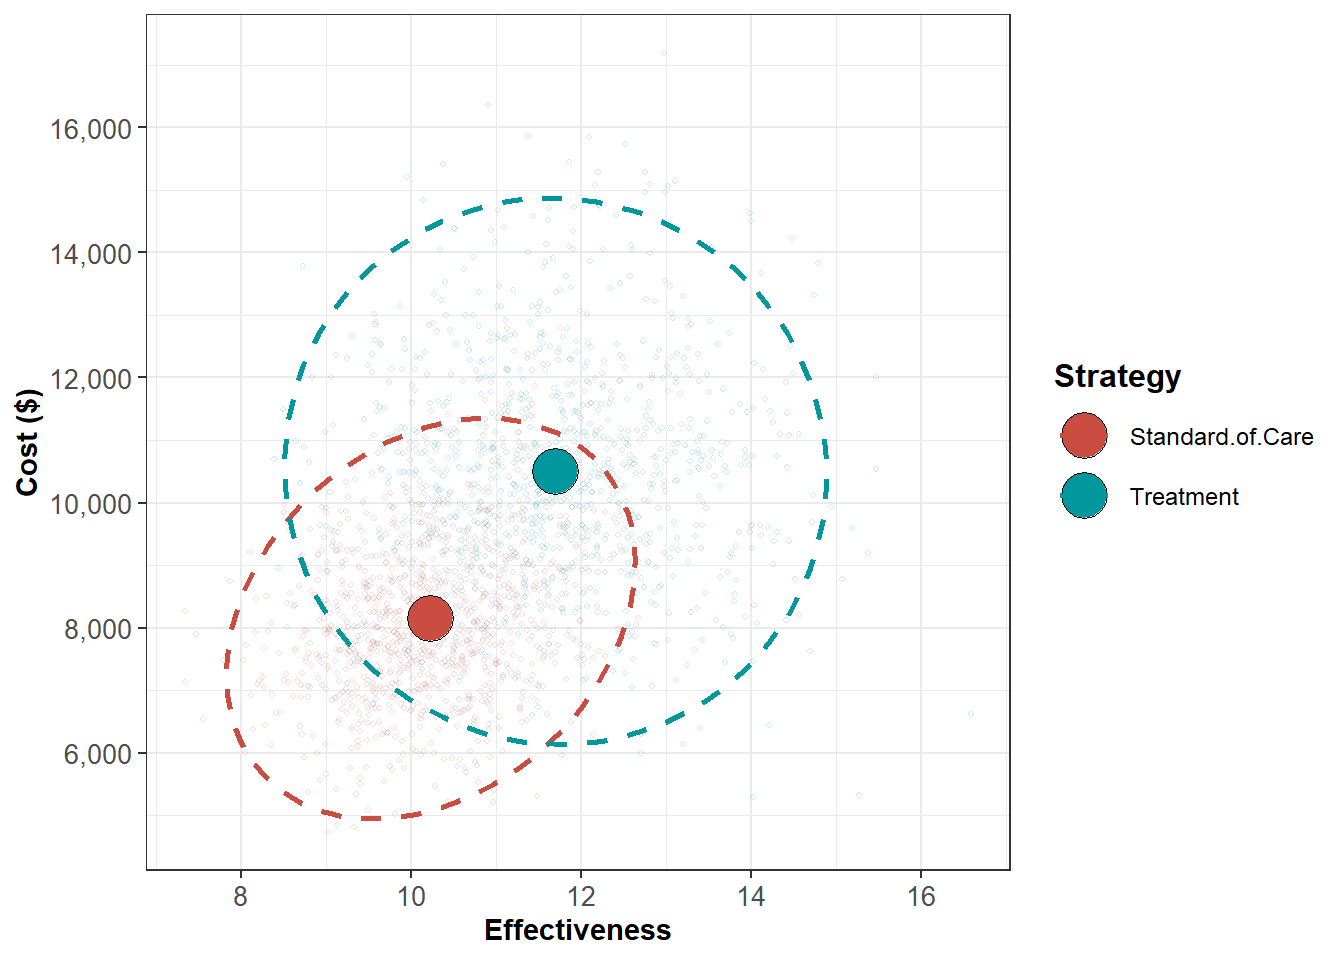
\includegraphics{markov_sick-sicker_PSA_solutions_files/figure-latex/unnamed-chunk-34-1.pdf}

\hypertarget{conduct-cea-with-probabilistic-output}{%
\subsection{09.4 Conduct CEA with probabilistic
output}\label{conduct-cea-with-probabilistic-output}}

\begin{Shaded}
\begin{Highlighting}[]
\CommentTok{# Compute expected costs and effects for each strategy from the PSA}
\NormalTok{df_out_ce_psa <-}\StringTok{ }\KeywordTok{summary}\NormalTok{(l_psa)}

\CommentTok{# Calculate incremental cost-effectiveness ratios (ICERs)}
\NormalTok{df_cea_psa <-}\StringTok{ }\KeywordTok{calculate_icers}\NormalTok{(}\DataTypeTok{cost       =}\NormalTok{ df_out_ce_psa}\OperatorTok{$}\NormalTok{meanCost, }
                              \DataTypeTok{effect     =}\NormalTok{ df_out_ce_psa}\OperatorTok{$}\NormalTok{meanEffect,}
                              \DataTypeTok{strategies =}\NormalTok{ df_out_ce_psa}\OperatorTok{$}\NormalTok{Strategy)}
\NormalTok{df_cea_psa}
\end{Highlighting}
\end{Shaded}

\begin{verbatim}
##       Strategy     Cost   Effect Inc_Cost Inc_Effect     ICER Status
## 1 No.Treatment  77033.8 15.69937       NA         NA       NA     ND
## 2    Treatment 143354.8 16.27791    66321  0.5785414 114634.8     ND
\end{verbatim}

\begin{Shaded}
\begin{Highlighting}[]
\CommentTok{# Save CEA table with ICERs}
\CommentTok{# As .RData}
\KeywordTok{save}\NormalTok{(df_cea_psa, }
     \DataTypeTok{file =} \StringTok{"markov_sick-sicker_probabilistic_CEA_results.RData"}\NormalTok{)}
\CommentTok{# As .csv}
\KeywordTok{write.csv}\NormalTok{(df_cea_psa, }
          \DataTypeTok{file =} \StringTok{"markov_sick-sicker_probabilistic_CEA_results.csv"}\NormalTok{)}
\end{Highlighting}
\end{Shaded}

\hypertarget{plot-cost-effectiveness-frontier}{%
\subsection{09.4.1 Plot cost-effectiveness
frontier}\label{plot-cost-effectiveness-frontier}}

\begin{Shaded}
\begin{Highlighting}[]
\KeywordTok{plot}\NormalTok{(df_cea_psa)}
\end{Highlighting}
\end{Shaded}

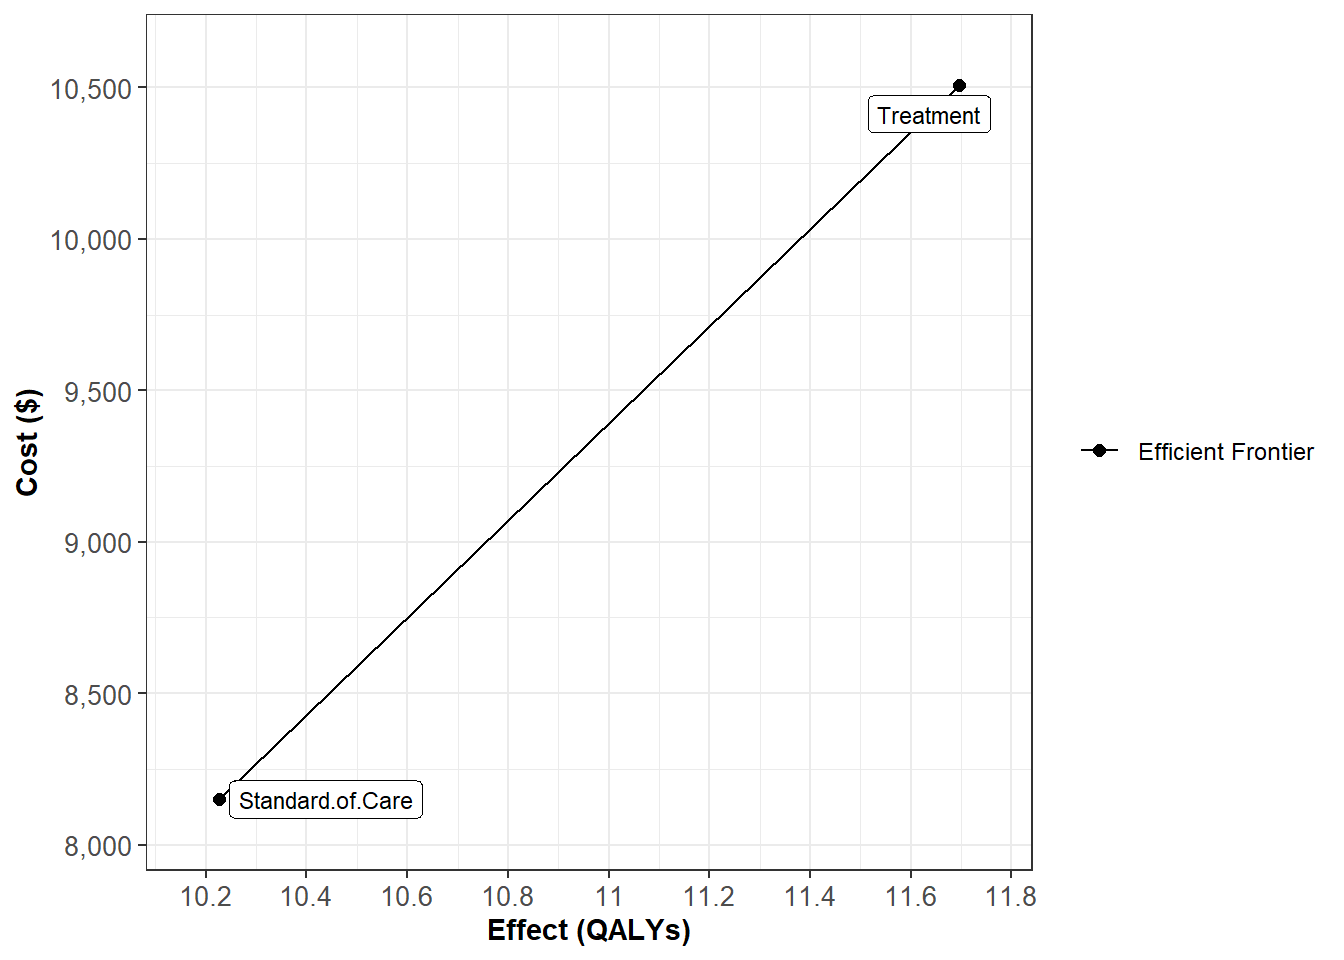
\includegraphics{markov_sick-sicker_PSA_solutions_files/figure-latex/unnamed-chunk-36-1.pdf}

\hypertarget{cost-effectiveness-acceptability-curves-ceacs-and-frontier-ceaf}{%
\subsection{09.4.2 Cost-effectiveness acceptability curves (CEACs) and
frontier
(CEAF)}\label{cost-effectiveness-acceptability-curves-ceacs-and-frontier-ceaf}}

\begin{Shaded}
\begin{Highlighting}[]
\NormalTok{ceac_obj <-}\StringTok{ }\KeywordTok{ceac}\NormalTok{(}\DataTypeTok{wtp =}\NormalTok{ v_wtp, }\DataTypeTok{psa =}\NormalTok{ l_psa)}
\CommentTok{# Regions of highest probability of cost-effectiveness for each strategy}
\KeywordTok{summary}\NormalTok{(ceac_obj)}
\end{Highlighting}
\end{Shaded}

\begin{verbatim}
##   range_min range_max cost_eff_strat
## 1         0    120000   No.Treatment
## 2    120000    200000      Treatment
\end{verbatim}

\begin{Shaded}
\begin{Highlighting}[]
\CommentTok{# CEAC & CEAF plot}
\KeywordTok{plot}\NormalTok{(ceac_obj)}
\end{Highlighting}
\end{Shaded}

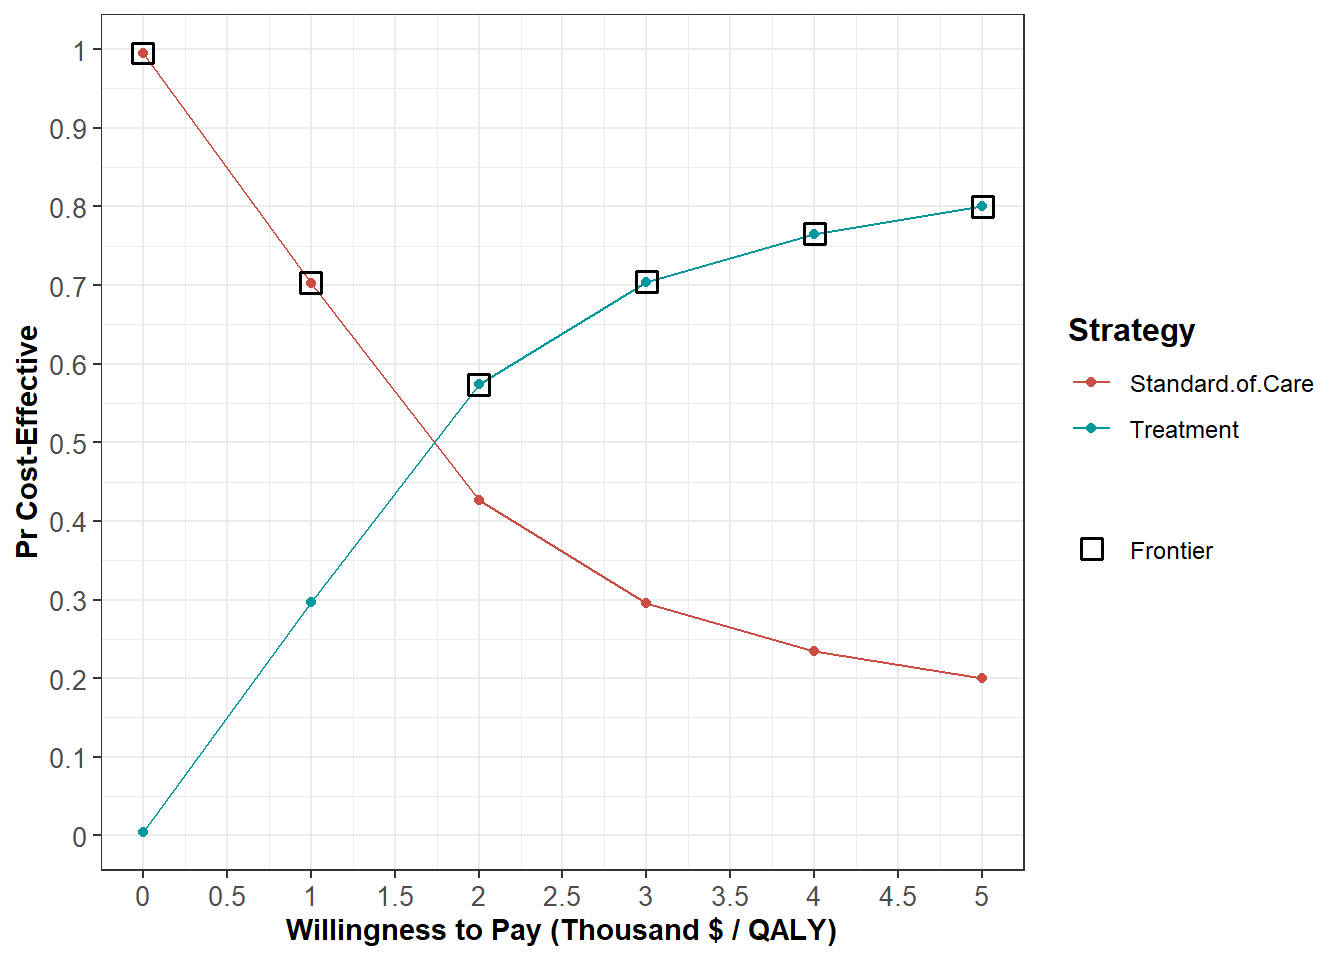
\includegraphics{markov_sick-sicker_PSA_solutions_files/figure-latex/unnamed-chunk-37-1.pdf}

\hypertarget{expected-loss-curves-elcs}{%
\subsection{09.4.3 Expected Loss Curves
(ELCs)}\label{expected-loss-curves-elcs}}

The expected loss is the the quantification of the foregone benefits
when choosing a suboptimal strategy given current evidence.

\begin{Shaded}
\begin{Highlighting}[]
\NormalTok{elc_obj <-}\StringTok{ }\KeywordTok{calc_exp_loss}\NormalTok{(}\DataTypeTok{wtp =}\NormalTok{ v_wtp, }\DataTypeTok{psa =}\NormalTok{ l_psa)}
\CommentTok{# ELC plot}
\KeywordTok{plot}\NormalTok{(elc_obj, }\DataTypeTok{log_y =} \OtherTok{FALSE}\NormalTok{)}
\end{Highlighting}
\end{Shaded}

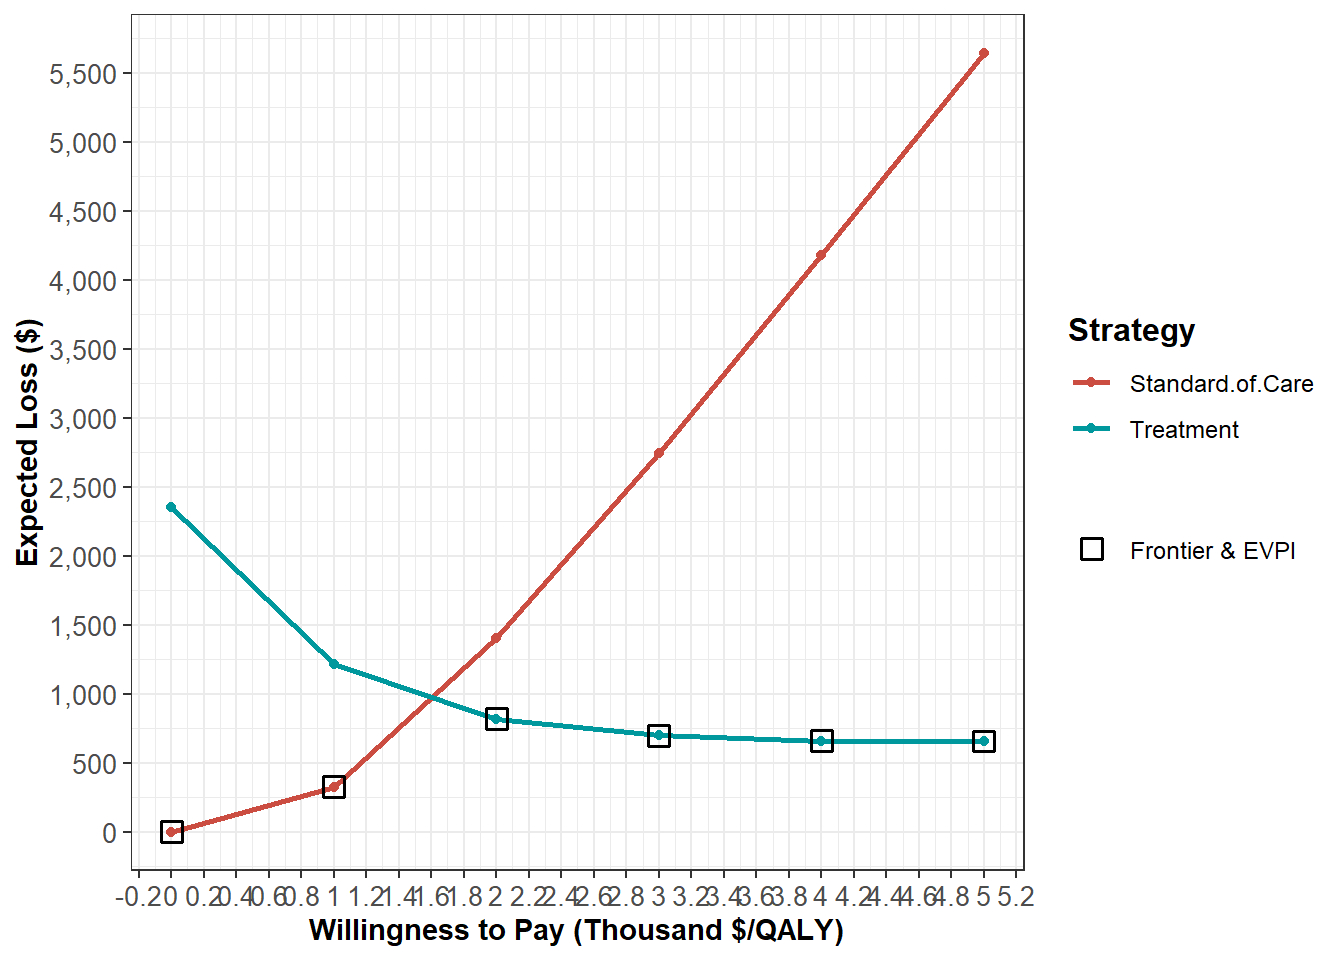
\includegraphics{markov_sick-sicker_PSA_solutions_files/figure-latex/unnamed-chunk-38-1.pdf}

\hypertarget{expected-value-of-perfect-information-evpi}{%
\subsection{09.4.4 Expected value of perfect information
(EVPI)}\label{expected-value-of-perfect-information-evpi}}

\begin{Shaded}
\begin{Highlighting}[]
\NormalTok{evpi <-}\StringTok{ }\KeywordTok{calc_evpi}\NormalTok{(}\DataTypeTok{wtp =}\NormalTok{ v_wtp, }\DataTypeTok{psa =}\NormalTok{ l_psa)}
\CommentTok{# EVPI plot}
\KeywordTok{plot}\NormalTok{(evpi, }\DataTypeTok{effect_units =} \StringTok{"QALY"}\NormalTok{)}
\end{Highlighting}
\end{Shaded}

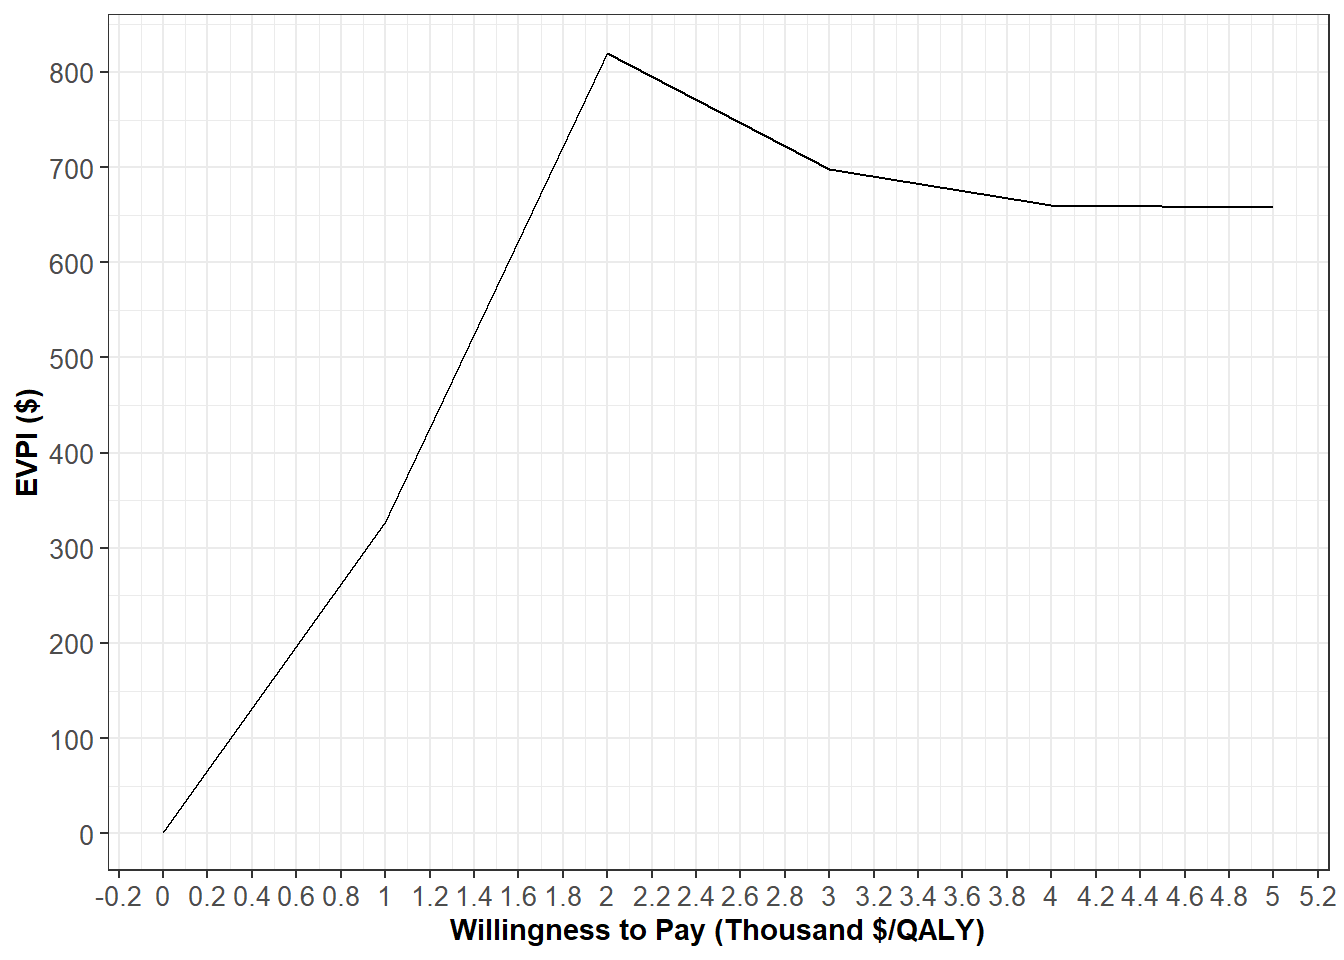
\includegraphics{markov_sick-sicker_PSA_solutions_files/figure-latex/unnamed-chunk-39-1.pdf}

\hypertarget{expected-value-of-partial-perfect-information-evppi}{%
\subsection{07.4.5 Expected value of partial perfect information
(EVPPI)}\label{expected-value-of-partial-perfect-information-evppi}}

\begin{Shaded}
\begin{Highlighting}[]
\NormalTok{evppi <-}\StringTok{ }\KeywordTok{calc_evppi}\NormalTok{(}\DataTypeTok{psa =}\NormalTok{ l_psa, }
                    \DataTypeTok{wtp =}\NormalTok{ v_wtp, }
                    \DataTypeTok{params =} \KeywordTok{c}\NormalTok{(}\StringTok{"p_S1S2"}\NormalTok{), }
                    \DataTypeTok{outcome =} \KeywordTok{c}\NormalTok{(}\StringTok{"nmb"}\NormalTok{),}
                    \DataTypeTok{type =} \KeywordTok{c}\NormalTok{(}\StringTok{"gam"}\NormalTok{, }\StringTok{"poly"}\NormalTok{),}
                    \DataTypeTok{poly.order =} \DecValTok{2}\NormalTok{,}
                    \DataTypeTok{k =} \DecValTok{-1}\NormalTok{,}
                    \DataTypeTok{pop =} \DecValTok{1}
\NormalTok{)}
\CommentTok{# EVPPI plot}
\NormalTok{dampack}\OperatorTok{:::}\KeywordTok{plot.evppi}\NormalTok{(evppi)}
\end{Highlighting}
\end{Shaded}

\includegraphics{markov_sick-sicker_PSA_solutions_files/figure-latex/unnamed-chunk-40-1.pdf}

\end{document}
